


%%%%%%%%%%%%%%%%%%%%%%%%%%%%%%%%%%%%%%%%%%%%%%%%%%%%%%%%%%%%%
%% HEADER
%%%%%%%%%%%%%%%%%%%%%%%%%%%%%%%%%%%%%%%%%%%%%%%%%%%%%%%%%%%%%
\documentclass[a4paper,twoside,11pt]{report}
\usepackage{a4}

\title{Entwicklung und Fertigung eines selbstfahrenden Modellautos}
\author{Felix Sandri, Philipp Kaltenleitner, Mert Guerel, David Petrovic}

\usepackage[text={150mm,240mm},bindingoffset=1cm]{geometry}

%% Deutsche Anpassungen %%%%%%%%%%%%%%%%%%%%%%%%%%%%%%%%%%%%%
\usepackage[ngerman]{babel}
\usepackage[T1]{fontenc}
\usepackage[ansinew]{inputenc}

\usepackage{lmodern} %Type1-Schriftart f�r nicht-englische Texte
\usepackage{color}
\usepackage{xcolor}

\usepackage{array} %F�r die Eidesstattliche Erkl�rung
\usepackage{float} %Fliegende Abbildungen / Objekte
\usepackage[margin=10pt,labelfont=bf,singlelinecheck=false]{caption}

\usepackage{hyperref}	%Querverweise
\usepackage{inputenc} 

\usepackage{fancyhdr} %Kopf- und Fu�zeile
\usepackage{lastpage} %letzte Seite referenzierbar
\usepackage{scrlayer}	%Page-Styles

%% Packages f�r Grafiken & Abbildungen %%%%%%%%%%%%%%%%%%%%%%
\usepackage{graphicx} %Zum Laden von Grafiken

%% Packages f�r Formeln %%%%%%%%%%%%%%%%%%%%%%%%%%%%%%%%%%%%%
\usepackage{amsmath}
\usepackage{amsthm}
\usepackage{amsfonts}

\usepackage{tocloft}	%Package to change TOC Style

\renewcommand{\footrulewidth}{0.4pt} %%Linie �ber Kopf / Fu�zeile

\renewcommand{\thechapter}{%	%%Change Chapter Numbering to roman
    \Roman{chapter}%
}

\counterwithout{section}{chapter}	%%Dont count chapters in in sections

\setlength{\cftchapnumwidth}{3em}	%%Add Space after Chapter TOC Numbering



%%%%%%%%%%%%%%%%%%%%%%%%%%%%%%%%%%%%%%%%%%%%%%%%%%%%%%%%%%%%%
%% DOKUMENT
%%%%%%%%%%%%%%%%%%%%%%%%%%%%%%%%%%%%%%%%%%%%%%%%%%%%%%%%%%%%%
\begin{document}

\fancyhead[RO,LE]{2023/24}
\fancyhead[C]{Abteilung f�r Elektrotechnik} 
\fancyhead[RE,LO]{\parbox[c]{30mm}{%
    \includegraphics[width=\linewidth]{./Abbildungen/HTBLuVA_Salzburg_Logo_RGB.jpg}
}}

\fancyfoot[RO,LE]{\thepage}
\fancyfoot[C]{Sandri, Kaltenleitner, G�rel, Petrovic}
\fancyfoot[RE,LO]{5BHET}
\setlength{\headheight}{38pt}

%%%%%%%%%%%%%%%%%%%%%%%%% WICHTIG!
\fancypagestyle{plain}{}    %% Kapitel-Anfangsseiten habe einen Plain-Stil darum wird keine
														%% Kopf/Fu�zeile angezeigt. Dieser Befehl verhindert dies
%%%%%%%%%%%%%%%%%%%%%%%%% WICHTIG!

\pagestyle{empty} %%Keine Kopf-/Fusszeilen auf den ersten Seiten.

%% Deckblatt %%%%%%%%%%%%%%%%%%%%%%%%%%%%%%%%%%%%%%%%%%%%%%%%
% Beginn - Formatierung der Titelseite

\vspace*{3pt}
\parbox[c]{80mm}{
	\begin{Large}\textbf{HTBLuVA Salzburg }\end{Large} \newline
	\textbf{H�here Lehranstalt f�r Elektrotechnik} \newline
	Ausbildungsschwerpunkt: \newline Energiesysteme und Industrieelektronik
}
\hfill
\parbox[c]{60mm}{  
	\includegraphics[width=\linewidth]{./Abbildungen/HTBLuVA_Salzburg_Logo_RGB.jpg}
}
\hrule\relax

\vspace*{30mm}
\begin{center} 
\begin{Huge}\textbf{Diplomarbeit}\end{Huge} \par \bigskip 
\begin{Large}5BHET 2023/24 \par \bigskip 
H�here Technische Bundeslehr- und Versuchsanstalt Salzburg \par \bigskip 
Abteilung f�r Elektrotechnik\end{Large} 
\vspace*{20mm}

%		In der Hautpdatei nach \usepackage{a4} folgendes Einf�gen:
%		\title{Entwicklung einer Diplomarbeitsvorlage}

\begin{huge}
	\makeatletter
	\textbf{\@title \\[1ex]}
	\makeatother
\end{huge}
\end{center}

\vspace{3cm}
\parbox[c]{60mm}{%
	\textbf{Ausgef�hrt von:}\par
	Felix Sandri\\
	Philipp Kaltenleitner\\	
	Mert G�rel\\
	David Petrovic\\
}%
\hfill%
\parbox[c]{70mm}{%
	\textbf{Betreuer}:\par
	BSc Simon Dantendorfer\\
	Prof. Dipl.-Ing. Reinhold Benedikter\\
	Prof. Dipl.-Ing. Robert Fuchs\\
	Prof. Dipl.-Ing. Timo Huemer\\
}%

\newpage
% Ende - Formatierung der Titelseite 

%% Eidesstattliche Erkl�rung %%%%%%%%%%%%%%%%%%%%%%%%%%%%%%%%
\newpage
\pagenumbering{Roman}
\vspace*{0cm}
\begin{center}
\textbf{\Huge{Eidesstattliche Erkl�rung}}
\end{center}
\vspace{1cm}
Wir erkl�ren an Eides statt, dass wir die vorliegende Arbeit selbstst�ndig und ohne fremde Hilfe verfasst, andere als die angegebenen Quellen nicht benutzt und die den benutzten Quellen w�rtlich und inhaltlich entnommenen Stellen als solche kenntlich gemacht haben.\\
Wir versichern, dass wir dieses Diplomarbeitsthema bisher weder im In- noch im Ausland (einer Beurteilerin oder einem Beurteiler) in irgendeiner Form als Pr�fungsarbeit vorgelegt haben.

% \usepackage{array} is required
\vspace*{3cm}
\begin{center}
\begin{tabular}{
	>{\centering\arraybackslash}p{4cm}
	>{\centering\arraybackslash}p{4cm}
	>{\centering\arraybackslash}p{4cm}}
            \hrulefill         &  & \hrulefill      \\
            Felix Sandri       &  & Philipp Kaltenleitner     \vspace*{1.5cm}\\ 
            \hrulefill         &  & \hrulefill      \\
            Mert G�rel         &  & David Petrovic            \vspace*{2cm}\\
            & \hrulefill & \\
            & Ort, Datum & \\
\end{tabular} 
\end{center}
	

%% Vorwort %%%%%%%%%%%%%%%%%%%%%%%%%%%%%%%%%%%%%%%%%%%%%%%%%%
\newpage
\pagestyle{fancy}
\chapter{Vorwort}
	TEST \cite{Kaltenleitner2019}

%% Abstract %%%%%%%%%%%%%%%%%%%%%%%%%%%%%%%%%%%%%%%%%%%%%%%%%
\newpage
\textbf{\Huge{Diplomarbeitsdokumentation}}

\begin{tabular}{|m{4.5cm}|m{9cm}|}															%senkrechter Strich steht f�r horizontale Linien
																																%mit m k�nnen die Gr��en der Zellen bestimmt werden
		\hline																											% \hline f�r eine horizontale Linie in der Tabelle
		& \\																												% mit & werden die Zellen abgerentzt
		Verfasser & Felix Sandri, Philipp Kaltenleitner, \\	% \\ steht f�r einen Zeilenumbruch in einer Tabelle
							& Mert G�rel, David Petrovic  \\ 
		& \\				
		\hline
		& \\
		Jahrgang Schuljahr & 5BHET \\ & 2023/24  \\ 								
		& \\ 			
		\hline
		
		& \\
		Thema der & Entwicklung und Fertigung eines selbstfahrenden \\ 
		Diplomarbeit & Modelautos\\ 
		& \\ 
		\hline
		& \\
		Kooperationspartner & HTBLuVA Salzburg \\ 
												& Kyocera AVX \\
											  & Mean Well/ Pro Connect \\ 
												& WG Global GmbH\\
												& SDP Automobile\\	
												& Mario's Autoteile\\	
												& Innovation Salzburg Pioniergarage GmbH\\ 
												& Schraubenking GmbH\\	
												
		& \\
		\hline \hline
		
		& \\
		Aufgabenstellung & Das Ziel besteht darin, ein Modellauto zu entwickeln, welches auf dem Gel�nde der HTBLuVA Salzburg autonom fahren kann. Hierf�r wird ein Auto von Grund auf neu konstruiert, inklusive aller mechanischen, elektronischen und softwaretechnischen Komponenten. Des Weiteren soll das Fahrzeug in allen mechanischen und elektrotechnischen Aspekten voll funktionsf�hig sein.
		\\
		& \\ 
		\hline \hline
		& \\
		
		Realisierung & Um das autonome Fahren zu erm�glichen, wird ein vollst�ndig neues Fahrzeug mit allen erforderlichen mechanischen Komponenten entwickelt, das ausreichend Platz bietet, um s�mtliche Elektronik unterzubringen. Zur Umgebungserfassung nutzt Athena einen LiDAR-Sensor sowie acht weitere Ultraschallsensoren. Die Hauptrecheneinheit ist ein Lattepanda 3 Delta, der zudem �ber eine Dual Edge TPU verf�gt, was eine schnellere Verarbeitung der Sensordaten erm�glicht. Durch k�nstliche Intelligenz kann Athena nicht nur die Daten verarbeiten, sondern auch das Fahrzeug steuern. Zus�tzlich wird ein ESP32 als Sub-Prozessor verwendet.\\
		 
		& \\ 
		\hline
		
		\end{tabular}	
		
		\pagebreak
				
		\begin{tabular}{|m{4.5cm}|m{9cm}|}
		
		\hline
		& \\
		Abbildung & \includegraphics[width=8.5cm]{./4_Mechanik/Abbildungen/Aufbau_Anleitung_render/Athena_fertig_4}\\ 
		& \\
		\hline 
	
		\end{tabular}	
		
		\begin{tabular}{|m{4.5cm}|m{9cm}|}
		
		\hline
		Ergebnisse & Das Modellauto Athena wurde sowohl mechanisch als auch in Bezug auf Hardware und Software rechtzeitig fertiggestellt und erfolgreich in Betrieb genommen. \\ 
		\hline
		
		\end{tabular}
		
		\begin{tabular}{|m{4.5cm}|m{9cm}|}\hline
		
		M�glichkeit der Einsichtnahme in die Arbeit & Die Diplomarbeit ist in gebundener Form in der
																									Schulbibliothek als auch bei AV Prof. Dipl-Ing.
																									(FH) Roland Holzer einzusehen. Dar�ber hinaus besitzt
																									jedes Mitglied des Projektteams eine vollst�ndige Version 
																									in gebundener und digitaler Form. \\ 
		\hline  
		
		\end{tabular}
		
		\begin{tabular}{|m{4.5cm}|m{4.28cm}|m{4.28cm}|}	%letzte Zeile muss in 3 Spalten unterteilt werden
		
		\hline
		
		Approbation & Pr�fer/Pr�ferin & Abteilungsvorstand \\ 
		(Datum/Unterschrift) &  & 	\\  
		&	& \\ 
		\hline

		\end{tabular}					%Ende der Tabelle
		\newpage
		
		
		
		
		
		
		
		\textbf{\Huge{Diploma Thesis Documentation}}

\begin{tabular}{|m{4.5cm}|m{9cm}|}															%senkrechter Strich steht f�r horizontale Linien
																																%mit m k�nnen die Gr��en der Zellen bestimmt werden
		\hline																											% \hline f�r eine horizontale Linie in der Tabelle
		& \\																												% mit & werden die Zellen abgerentzt
		Authors & Felix Sandri, Philipp Kaltenleitner, \\	% \\ steht f�r einen Zeilenumbruch in einer Tabelle
							& Mert G�rel, David Petrovic  \\
		& \\				
		\hline
		& \\
		Form Academic year & 5BHET \\ & 2023/24  \\ 								
		& \\ 			
		\hline
		
		& \\
		Topic & Development and Manufacturing of a Self-Driving\\ 
					& Model Car\\ 
		& \\ 
		
		\hline
		
		& \\
		Co-operation  			& HTBLuVA Salzburg \\ 
												& Kyocera AVX \\
											  & Mean Well/ Pro Connect \\ 
												& WG Global GmbH\\
												& SDP Automobile\\	
												& Mario's Autoteile\\	
												& Innovation Salzburg Pioniergarage GmbH\\ 
												& Schraubenking GmbH\\	
												
		& \\
		\hline \hline
		& \\
	Assignment of Tasks & The goal is to develop a model car capable of autonomous driving on the premises of HTBLuVA Salzburg. To achieve this, a car will be completely designed from scratch, including all mechanical, electronic, and software components. Furthermore, the vehicle is intended to be fully functional in all mechanical and electrical aspects. \\
		& \\ 
		\hline \hline
		& \\
		 
		Realization & To enable autonomous driving, a completely new vehicle is being developed with all necessary mechanical components, providing ample space to accommodate all electronics. Athena utilizes a LiDAR sensor and eight additional ultrasonic sensors for environment mapping. The main computing unit is a Lattepanda 3 Delta, equipped with a Dual Edge TPU for faster sensor data processing. Through artificial intelligence, Athena can not only process data but also control the vehicle. Additionally, an ESP32 is used as a sub-processor. \\
		 
		& \\ 
		\hline
		
		\end{tabular}	
		
		\begin{tabular}{|m{4.5cm}|m{9cm}|}
		
		\hline
		
		& \\
		Illustrative Graph & \includegraphics[width=8.5cm]{./4_Mechanik/Abbildungen/Aufbau_Anleitung_render/Athena_fertig_4}\\ 
		& \\
		
		\hline 
	
		\end{tabular}	
		
		\begin{tabular}{|m{4.5cm}|m{9cm}|}
		
		\hline
		Results & The model car Athena has been completed on time, both mechanically and in terms of hardware and software, and has been successfully put into operation. \\ 
		\hline
		
		\end{tabular}
		
		\begin{tabular}{|m{4.5cm}|m{9cm}|}\hline
		
		Accessibility of \newline Diploma Thesis	 		& 		The diploma thesis is available in the school library
																												as well as in the office of the head of department
																												Prof. Dipl-Ing. (FH) Roland Holzer. In addition,
																												each member of the project team has a complete
																												version in hardcover and digital form.\\ \hline  
		
		\end{tabular}
		
		\begin{tabular}{|m{4.5cm}|m{4.28cm}|m{4.28cm}|}	%letzte Zeile muss in 3 Spalten unterteilt werden
		
		\hline
		Approval & Examiner & Head of department \\ 
		(Date/Sign) &  & 	\\  
		& & \\ 
		\hline
		\end{tabular}					%Ende der Tabelle
		\newpage

%% Inhaltsverzeichnis %%%%%%%%%%%%%%%%%%%%%%%%%%%%%%%%%%%%%%%
\clearpage
\tableofcontents %Inhaltsverzeichnis
\cleardoublepage %Das erste Kapitel soll auf einer ungeraden Seite beginnen.

\pagenumbering{arabic}

%% Einf�hrung %%%%%%%%%%%%%%%%%%%%%%%%%%%%%%%%%%%%%%%%%%%%%%%
\newpage
\chapter{Einf�hrung}
	
	\section{Projektteam}
	
		\begin{figure}[H]
    \centering
    \begin{minipage}[b]{0.48\textwidth}
        \centering
        \includegraphics[scale=0.12]{./1_Einfuehrung/Abbildungen/Felix}
        \caption{Felix Sandri}
    \end{minipage}
    \begin{minipage}[b]{0.48\textwidth}
        \centering
        \includegraphics[scale=0.12]{./1_Einfuehrung/Abbildungen/Philipp}
        \caption{Philipp Kaltenleitner}
    \end{minipage}
	\end{figure}
	\begin{figure}[H]
    \centering
    \begin{minipage}[b]{0.48\textwidth}
        \centering
        \includegraphics[scale=0.12]{./1_Einfuehrung/Abbildungen/Mert}
        \caption{Mert G�kay G�rel}
    \end{minipage}
    \begin{minipage}[b]{0.48\textwidth}
        \centering
        \includegraphics[scale=0.12]{./1_Einfuehrung/Abbildungen/David}
        \caption{David Petrovic}
    \end{minipage}
	\end{figure}
\newpage

\section{Projektbetreuer}
	\begin{itemize}
		\item \textbf{Prof. Dipl.-Ing. Robert Fuchs} unterst�tzte Felix Sandri beim fertigen und implementieren des elektrischen Antriebssystems.
		\item \textbf{Prof. Dipl.-Ing. Reinhold Benedikter} war stets eine gro�e Unterst�tzung w�hrend dem gesamten Verlauf des Projekts, er half beim Bestellen aller Komponenten und unterst�tzte Philipp Kaltenleitner erheblich beim �berarbeiten der Aufh�ngung und Lenkung.
		\item \textbf{BSc Simon Dantendorfer} unterst�tzte Mert G�rel bei Fragen bez�glich Optimierung der Software und Implementierung der ROS-Entwicklungsumgebung.
		\item \textbf{Prof. Dipl.-Ing. Timo Huemer} betreute David Petrovic bez�glich der Vorgehensweise w�hrend der Softwareentwicklung und dem Designprozess der Website.
	\end{itemize}

\section{Aufgabenteilung}

%% Einleitung %%%%%%%%%%%%%%%%%%%%%%%%%%%%%%%%%%%%%%%%%%%%%%%
\newpage
\chapter{Einleitung}
	
\section{Motivation}
	
Der Grundstein f�r Athena wurde in der zweiten Klasse gelegt. Es sollte ein CAD-Projekt im Fach CPE erstellt werden. Aufgrund unserer gro�er Automobilaffinit�t entschieden man sich f�r ein ferngesteuertes Auto. Da es in der zweiten Klasse jedoch nicht m�glich war, ein so komplexes Projekt zu fertigen, beschlossen wir, es weiterzuentwickeln.\\
\\
Um mehr in den Bereich Elektrotechnik einzutauchen, wurde ein Konzept f�r ein selbstfahrendes Auto entwickelt. Dieser Bereich ist derzeit besonders interessant, da viele gro�e Automobilhersteller bereits am autonomen Fahren arbeiten.\\
\\
In der vierten Klasse bot sich die M�glichkeit, dieses Projekt umzusetzen. Da dies aufgrund von Budgetknappheit und langen Lieferzeiten nicht m�glich war, wurde das Projekt in der f�nften Klasse als Diplomarbeit weitergef�hrt. Das Ziel war es, dieses Projekt nach jahrelanger Arbeit erfolgreich abzuschlie�en.

\section{Zielsetzung}

Die Zielsetzung f�r Athena besteht darin, ein innovatives und vollst�ndig autonomes Modellauto zu entwickeln, welches die Schulumgebung pr�zise kartieren und intelligent navigieren kann. Durch die Integration von K�nstlicher Intelligenz soll ein Fahrzeug geschaffen werden, das nicht nur in der Lage ist, Hindernisse zu erkennen und zu umgehen, sondern auch effiziente Routen innerhalb des Schulumfeldes planen kann.


\section{Aufbau}

Die Diplomarbeit ist in zwei �bergeordnete Bereiche unterteilt, wobei der praktische Teil drei spezifische Bereiche umfasst:\\

Im theoretischen Hauptteil erl�utern alle Autoren die grundlegende Theorie, die ihre Arbeit informiert. Dabei pr�sentiert jeder Autor eine umfassende Darstellung der theoretischen Grundlagen. Jeder Autor bietet eine ausf�hrliche Darstellung der theoretischen Grundlagen, die als Basis f�r ihre Arbeit dienen.\\

Die Unterbereiche umfassen:

\begin{itemize}
\item Elektronik
\item Mechanik
\item Software
\end{itemize}

Innerhalb der Arbeit werden die Elektronik, Mechanik und Software des Fahrzeugs behandelt. Dabei wird ein spezifischer Fokus auf elektronische Komponenten wie Motoren sowie auf mechanische Aspekte wie die Aufh�ngung gelegt. Die Softwareanalyse konzentriert sich auf die Programmierung des Fahrzeugs.


%% Stand der Technik %%%%%%%%%%%%%%%%%%%%%%%%%%%%%%%%%%%%%%%%
\newpage
\chapter{Stand der Technik}
	
	\section{3D-Druck}
	\fancyfoot[C]{G�rel}
	\fancyfoot[C]{G�rel}
\subsection{3D-Druck und FDM-Druckverfahren}

Der 3D-Druck, auch als additive Fertigung bekannt, hat sich zu einer weit verbreiteten Technologie entwickelt, die in verschiedenen Branchen und Anwendungen eingesetzt wird. Ein g�ngiges Verfahren im 3D-Druck ist das Fused Deposition Modeling (FDM), auch bekannt als Fused Filament Fabrication (FFF). Hierbei wird thermoplastisches Filament durch eine beheizte D�se extrudiert und Schicht f�r Schicht aufgetragen, um das gew�nschte Objekt zu erstellen.

\paragraph{D�sengr��en im FDM-Druckverfahren}

\begin{itemize}
    \item \textbf{0,2 mm D�se:} Diese D�se erzeugt sehr feine Details und erm�glicht eine hohe Pr�zision beim Drucken. Sie eignet sich gut f�r Modelle mit filigranen Strukturen und kleinen Oberfl�chendetails. Allerdings dauert der Druck mit einer 0,2 mm D�se in der Regel l�nger, da d�nnere Schichten gedruckt werden m�ssen.
    
    \item \textbf{0,4 mm D�se:} Dies ist die Standardd�sengr��e f�r die meisten FDM-3D-Drucker. Sie bietet ein ausgewogenes Verh�ltnis zwischen Druckgeschwindigkeit und Detailgenauigkeit. Die meisten 3D-Drucker werden mit einer 0,4 mm D�se ausgeliefert, da sie vielseitig einsetzbar ist und gute Ergebnisse liefert.
    
    \item \textbf{0,6 mm D�se:} Eine 0,6 mm D�se erm�glicht einen schnelleren Druck, da sie gr��ere Schichten auftr�gt und somit weniger Schichten f�r das gleiche Objekt ben�tigt werden. Dies f�hrt zu k�rzeren Druckzeiten, allerdings auf Kosten der Detailgenauigkeit. Sie eignet sich gut f�r Prototypen und Funktionsmodelle, bei denen eine hohe Druckgeschwindigkeit wichtiger ist als feine Details.
\end{itemize}

\paragraph{Unterschied zwischen normalen und geh�rteten D�sen}

\paragraph{Normale D�sen:} Normale D�sen bestehen in der Regel aus Messing oder Edelstahl und sind gut f�r den allgemeinen Gebrauch geeignet. Sie sind kosteng�nstig und bieten eine gute W�rmeleitf�higkeit, was f�r einen reibungslosen Filamentfluss w�hrend des Druckvorgangs wichtig ist. Allerdings k�nnen normale D�sen anf�llig f�r Verschlei� sein, insbesondere wenn abrasive Filamente wie zum Beispiel mit Kohlefaser verst�rktes PLA verwendet werden.

\paragraph{Geh�rtete D�sen:} Geh�rtete D�sen sind speziell behandelt, um widerstandsf�higer gegen�ber abrasiven Filamenten zu sein. Sie bestehen oft aus Stahllegierungen wie geh�rtetem Stahl oder Messing mit einer speziellen Beschichtung. Diese Beschichtung bietet eine zus�tzliche Schutzschicht gegen Verschlei� und verl�ngert die Lebensdauer der D�se. Geh�rtete D�sen sind ideal f�r den Druck mit abrasiven Materialien wie faserverst�rktem Kunststoff oder Metallfilamenten. Sie sind jedoch in der Regel teurer als normale D�sen.

	
	\newpage
	\fancyfoot[C]{Sandri}
	\subsection{Filamente des FDM-Drucks}
	Beim 3D-Druck spielt das verwendete Filament eine sehr gro�e Rolle. Durch die korrekte Auswahl dessen k�nnen sehr viele verschiedene mechanische Eigenschaften erreicht werden.
	\\
	\\
	Zum FDM-Druck werden Thermoplaste in Form einer Schnur auf eine Rolle aufgewickelt verwendet. Dieses Filament wird meist im Querschnitt 1,75mm und 2.85mm angeboten, in den letzten Jahren hat sich jedoch der Querschnit 1,75mm weitl�ufig durchgesetzt. Filament-Spulen sind meist in 1-Kilo-Inkrementen erh�ltlich.
	
	\subsubsection{Polylactid (PLA)}
		Polylactid, meist unter seiner Abk�rzung PLA bekannt, ist der am weitesten verbreitete Kunststoff im FDM-Druck. Er ist vorallem durch seine leichte Verarbeitung und geringen Preis weit verbreitet worden. Hergestellt wird PLA aus Pflanzenst�rke. PLA ist grunds�tzlich transparent, steif, �L-, Fett- und Alkoholbest�ndig und zugellasen f�r Lebensmittel. Jedoch ist es spr�de, nicht UV-best�ndig und leicht thermisch verformbar.\cite{kunststoffe.de2024}
		
	\subsubsection{Polyethylenterephthalat (PET/PETG/PETT)}
		Polyethylenterephthalat ist ein sehr weit verbreiteter Kunststoff, er ist aus allem von Recycling-Flaschen bis zu Textilfa�ern bekannt. Beim 3D-Druck wird reines PET eher selten verwendet, es wird die abge�nderte Variante PETG verwendet. Diese ist mit Glycol modifiziert und sorgt daf�r, dass das Material besser f�r den 3D-Druck geeignet wird. Es wird oft als bessere Alternative zu PLA betrachtet, da es haltbarer und flexibler als PLA ist aber immernoch sehr einfach zu drucken ist. Polyethylen-CoTrimethylen-Terephthalat (PETT) wird auch immer h�ufiger vorallem aufgrund von seiner Transparenz verwendet.\cite{all3dp.com2023}
	
	\subsubsection{Acrylnitril-Butadien-Styrol-Copolymer(ABS)}	
		Acrylnitril-Butadien-Styrol-Copolymer, auch unter ABS bekannt, ist der g�ngigste Werkstoff wenn 3D-Druck-Teile etwas widerstandsf�higer sein m�ssen. ABS hat hohe Festigkeit, eine h�here Temperaturbest�ndigkeit wie PLA und PETG und ist nicht spr�de. Jedoch ist es auch erheblich schwieriger zu drucken, da es dazu neigt sich beim Abk�hlen zu verformen, deshalb wird beim Drucken meist eine recht hohe Druckbetttemperatur von 80-110�C verwendet. Auch ein geschlossener Druckraum ist aus diesem Grund von Vorteil. Beim Druck enstehen auch D�mpfe die zu Kopfschmerzen oder �belkeit f�hren k�nnen, deswegen ist eine gute Entl�ftung beziehungsweise Filttrierung der Luft zu empfehlen.\cite{all3dp.com2023}
	
	\subsubsection{Thermoplastische Elastomere(TPE/TPU)}
		Thermoplastische Elastomere sind Kunststoffe mit Gummiartigen Eigenschaften, die sehr flexibel und sehr haltbar sind. TPU ist eines Sort von TPE, die etwas steifer und besser f�r den 3D-Druck geeignet ist. Sie k�nnen St��en und Ersch�tterungen wesentlich besser als PLA oder ABS standhalten.\cite{all3dp.com2023} TPU ist grunds�tzlich einfach zu drucken, St�tzsturkturen sollten jedoch weitgehend vermieden werden, da die klebrige und flexible Natur des Materials diese sehr schwierig zu entfernen macht. TPU ist auch wie viele andere Thermoplate hygroskopisch, wenn es vor dem Druck nicht ausreichend trocken ist, kann dies zu starkem Stringing, zur Fadenbildung f�hren.
	

	
	%\section{Fr�sen und Drehen}
	Test
	
	\fancyfoot[C]{Sandri}
\section{Laserschneiden}
	Beim Laserschneiden k�nnen meist flache Werkstoffe verschiedenster Dicke mithilfe von einem konzentrierten Laserstrahl ohne Ber�hrung geschnitten werden. Der Laserstrahl erhitzt dabei das Material an einem Punkt so stark, dass es sofort schmilzt oder verdampft. Mithilfe von einem Schneidgas kann das nun geschmolzene Material aus der Schnittfuge geblasen werden. Mit dieser Technik k�nnen eine Vielzahl an Materialien, wie zum Beispiel Holz, Acryl, Schaumstoff oder auch diverse Metalle wie Stahl, Edelstahl und Aluminium. \cite{Trumpf2024}
	
	\subsection{Arten von Lasern}
	Allgemein k�nnen Laser in f�nf unterschiedliche Typen unterteilt werden:
	\begin{itemize}
		
		\item Gaslaser
		\item Festk�rperlaser
		\item Diodenlaser
		\item Freie Elektronenlaser
		\item Farbstofflaser
		
	\end{itemize}
	Das Laseraktive Medium kann entweder durch das optische Pumpen (mit Licht), durch Strom oder durch einen chemischen Prozess angeregt werden.
	Es eignet sich jedoch nicht jeder Laser zur Materialverarbeitung.\cite{eval.at2024} Die in der Materialverarbeitung am verbreitensten Laser sind folgende:
	
	\subsubsection{CO2-Laser}
		Dies ist der in der Industrie am meist verbreiteste Gaslaser, andere Gaslaser z.B N2-Laser oder Excimerlaser haben eine �hnliche Funktionsweise, aber andere Eigenschafften. Durch Zufuhr von elektrischer Energie �ber Elektroden in ein Gasgemisch von ca. 70\% He, 20\% N2 und 10\% CO2 wird das Gas zun�chst in ein elektrisch leitendes Plasma verwandelt, welches anschlie�end durch eine Reihe von Spiegeln konzentriert und fokussiert wird. Da diese Laser einen Wirkungsgrad von maximal 15\% haben, sie bei hohen Leistungen eine sehr hohe Verlustleistung, die abgef�hrt werden muss. sie werden deswegen im Bereich von 10 bis 200Watt zum Schneiden und gravieren von d�nnen organischen Materialien wie Kunsstoffe, Holz oder Textilien verwendet.\cite{eval.at2024}
	
	\begin{figure}[H]
		\centering
		\includegraphics[scale=0.5]{./3_Stand_der_Technik/Abbildungen/Gaslaser_1}
		\caption{Aufbau eines Gaslasers\cite{eval.at2024}}
	\end{figure}
	
	\subsubsection{HeNe-Laser}
		Der HeNe Laser ist ein Gaslaser mit �hnlicher Funktionsweise zum CO2-Laser. �r wird meistens als Justierlaser verwendet, da er mit einer Leistung von unter 5mW einen sehr gut sichtbaren roten Laser erzeugt. Es sind auch andere Farben bzw Wellenl�ngen m�glich.\cite{eval.at2024}
		
	\subsubsection{Nd:YAG-Laser}
		Bei diesem Laser besteht das Lasermedium aus einem Kristall, die Energiezufuhr erfolgt durch Licht. Ein Nd:YAG-Laser(Neodym-dotierter Yttrium-Aluminium-Granat-Laser) emittiert meist eine infrarote Strahlung. Die Form dieses Kristalls ist meist in Stabform z.B. mit Durchmesser von 1cm und einer L�nge von 10cm. Er wird zwichen zwei Spiegeln positioniert und durch Blitzlampen oder Laserdionden angepumpt. Der mit Blitzlampen angepumpte Nd:YAG Laser is weiterhin der am meist verbreitete Festk�rperlaser. Ein gro�er Vorteil dieses Lasers ist auch, dass er sich im Gegensatz zum CO2-Laser durch eine Glasfa�er leiten l�sst und so f�r den Einsatz auf Roboterarmen geeignet ist.\cite{eval.at2024}
		
		\begin{figure}[H]
			\centering
			\includegraphics[scale=0.5]{./3_Stand_der_Technik/Abbildungen/NdYAGlaser_1}
			\caption{Aufbau eines Nd:YAG-Lasers\cite{eval.at2024}}
		\end{figure}
		
	\subsubsection{Faserlaser}
		Der Faserlaser besteht aus mehreren Metern lichtleitenden Faser, die mit laseraktiven Atomen dotiert sind. Durch den geringen Durchmeser dieser,(<100micrometer) erzeugt er nur Licht h�chster Strahlqualit�t und erreicht eine Effizienz von bis zu 30\%.\cite{eval.at2024}
		
	\subsubsection{Diodenlaser}
		Der Diodenlaser funktionier aufgrund vom Prinzip des pn-�bergangs von Halbleitern. Er hat eine sehr kompakte Bauweise und einen sehr hohen Wirkungsgrad von bis zu 50\%. Er besitzt im Vergleich zu anderen Lasern jedoch schlechter Strahlenqualit�t und eignet sich so eher nicht zum Schneiden.\cite{eval.at2024}
		
		\begin{figure}[H]
			\centering
			\includegraphics[scale=0.5]{./3_Stand_der_Technik/Abbildungen/Diodenlaser_1}
			\caption{Aufbau eines Diodenlasers\cite{eval.at2024}}
		\end{figure}
	
	\subsection{Schneiden verschiedener Werkstoffe}
	Laserschneidmaschinen sind meistens CNC-Maschinen. Um ein gutes Ergebnis zu erhalten, gilt es die Maschine dem Material entsprechend gut einzustellen. Die wichtigsten Faktoren sind dabei die Laserleistung und die Schnittgeschwindigkeit. Die hochwertigsten Ergebnisse werden meistens mit wenig Leistung und wenig Geschwindigkeit erreicht, sind bei gro�en Werkst�cken jedoch oft unvorteilhaft. Es gilt also ein Gleichgewicht zwischen Geschwindigkeit und Qualit�t der Schnittkante zu erreichen. 
	Bei gr��eren Materialdicken wird meistens auf die Schnittkante ein Gas mit hohem Druck zugef�hrt, um geschmolzenes Material zu entfernen und die Schnittkante daran zu hindern sofort zu oxidieren. Daf�r werden meistens entweder Druckluft, O2 oder N2 verwendet. 
	Die Reihenfolge der Schnittkonturen sollte auch beachtet werden. Im Normalfall werden zuerst alle innenliegenden Konturen und dann die au�enliegende Kontur geschnitten.
	
	\newpage
	\fancyfoot[C]{Kaltenleitner}
\section{Mechanik}
	
	\subsection{Aufh�ngung}
	Wird bei Autos �ber die Aufh�ngung oder das Fahrwerk gesprochen, so meint man damit ein System von Komponenten, welches das Fahrzeug mit den R�dern verbindet. Die Hauptaufgaben einer Aufh�ngung sind:
	\begin{itemize}
	\item F�hrung: 	Die Aufh�ngung ist mitverantwortlich f�r die richtige F�hrung der R�der. Bei den meisten Automobilen sind nur die Vorderreifen gelenkt. Die Hinterreifen sollten m�glichst gerade gef�hrt sein. Es muss sichergestellt sein, dass die R�der in Kurven und bei Geradeausfahrt die richtige Richtung halten.
	\item Federung: 	Die Federung sorgt daf�r, dass das Auto auch bei unebenen Stra�enoberfl�chen stabil und kontrollierbar bleibt. Sie absorbiert die St��e und Vibrationen, die von Bodenunebenheiten hervorgerufen werden und verringert dadurch die �bertragung dieser Bewegungen auf die Karosserie des Fahrzeugs und der Insassen. Bei vereinzelten Fahrzeugen mit einer Starrachse gibt es diese nicht. 
	\item D�mpfung: Die D�mpfung reduziert die Schwingungen der Federung und verhindert, dass das Auto nach einer Unebenheit auf der Stra�e weiter schwingt. Sie sorgt f�r eine schnellere R�ckkehr des Rades in seine normale Position und hilft dabei, die Kontrolle �ber das Fahrzeug zu behalten.
	\item Lastenverteilung: Eine gute Aufh�ngung hilft auch dabei, das Gewicht des Fahrzeugs gleichm��ig auf alle R�der zu verteilen, was zu einer verbesserten Traktion und einem besseren Handling f�hrt.
	\end{itemize}
	Zusammengefasst ist die Aufgabe einer Aufh�ngung, eine sichere und komfortable Verbindung zur Stra�e herzustellen.
	
	\subsubsection{Arten von Aufh�ngungen}
		\paragraph{Starrachse}
		Die wohl �lteste Aufh�ngung ist eine Starrachse. Bei einer Starrachsen-Aufh�ngung sind die R�der an einer einzigen Achse miteinander verbunden. Das bedeutet, dass beide R�der an der Vorder- oder Hinterachse zusammen auf- und abfedern. In den ersten Ausf�hrungen wurde auf eine Federung komplett verzichtet. In sp�teren Jahren wurden zus�tzlich Blattfedern verbaut. Heute wird sie Gro�teiles in Kombination mit einer Luftfederung gebaut. Diese Art der Aufh�ngung wird noch heute in vielen LKWs, Traktoren und Gel�ndefahrzeugen verwendet. Diese Art der Aufh�ngung ist bekannt f�r ihre Einfachheit, Robustheit und gute Traktion, aber sie bietet oft einen geringeren Fahrkomfort im Vergleich zu moderneren unabh�ngigen Aufh�ngungssystemen. Die Starrachsen-Aufh�ngung ist also kosteng�nstig, einfach zu warten und bietet gute Traktion, jedoch oft auf Kosten des Fahrkomforts.\cite{Fahrwerktechnik_Grundlagen_2005} \cite{Palla2021}
	
		\begin{figure}[H]
			\centering
			\includegraphics[scale=1.4]{./3_Stand_der_Technik/Abbildungen/Starrachse_1}
			\caption{ BRIST RDD 45-175 Starrachse \cite{Bristaxle.com2023}}
		\end{figure}
		
		\begin{figure}[H]
			\centering
			\includegraphics[scale=1.4]{./3_Stand_der_Technik/Abbildungen/Starrachse_2}
			\caption{BRIST RFS 60-175 Starrachse\cite{Bristaxle.com2023}}
		\end{figure}
		
		\paragraph{Trailing Arm Suspension / Schr�glenkerachse}
		Die Schr�glenkerachse ist am einfachsten zu beschreiben, in dem man sie mit der Schwinge eines Motorrads vergleicht. Sie besteht aus zwei Schwingen, welche ein St�ck vor der Achse drehend gelagert und mit dem Chassis verbunden sind. Ein Sto�d�mpfer ist in der N�he der Achse mit der Schwinge und dem Radkasten verbunden. Diese Art der Aufh�ngung wurde haupts�chlich f�r die Hinterachse benutzt.
Sie ist g�nstig in der Entwicklung und Produktion neigt jedoch dazu bei zu starken Seitenkr�ften zu �bersteuern, weshalb sie heute als veraltet gilt. \cite{Fahrwerktechnik_Grundlagen_2005} \cite{Palla2021}

		\paragraph{Doppelquerlenker-Radaufh�ngung}
		Die Doppelquerlenker-Radaufh�ngung ist das kostenintensivste Fahrwerkskonzept, welches oft in Fahrzeugen mit h�heren Leistungsanforderungen oder einem Fokus auf Komfort und Fahrdynamik verwendet wird. Diese Aufh�ngung besteht aus zwei Querlenkern, die �ber und unter dem Radtr�ger befestigt sind. Der Sto�d�mpfer mit au�enliegender Feder (manchmal auch mit Luftfederung gefertigt) wird am unteren Querlenker und an dem Domlager (Montagepunkt im Radkasten) montiert. 
In vereinzelten F�llen gibt es auch ein sogenannte Push oder Pull-Rod Systeme. Diese werden nur im Rennsport oder bei Sportwagen benutzt. Hierbei liegen die D�mpfer im inneren des Autos und werden mit Hilfe einer Umlenkung und einer Stange zu den Querdenkern gef�hrt. Sie wird besonders gerne bei sogenannten �open-wheel-cars� benutzt. Damit sind Fahrzeuge gemeint wo die Reifen freistehen ohne Kotfl�gel sind.  Eine Push oder Pull-Rod-Aufh�ngung ist im Bereich des Fahrwerks platzsparender, erm�glicht pr�zise Einstellung des Fahrwerks und besitzt bessere aerodynamische Eigenschaften. Die Produktions- und Entwicklungskosten sind jedoch sehr hoch.
Die Doppelquerlenker-Aufh�ngung erm�glicht die unabh�ngige Arbeit jedes Lenkers. Dadurch bietet sie eine pr�zise Steuerung der Raddynamik. Die R�der k�nnen einzeln auf Unebenheiten reagieren, ohne dass die Bewegung des einen Rades die des anderen beeinflusst. Dies verbessert nicht nur die Stra�enlage und das Handling des Fahrzeugs, sondern auch den Fahrkomfort, da St��e und Unebenheiten besser absorbiert werden.
Die Anpassungsm�glichkeiten sind ebenfalls ein Pluspunkt dieser Aufh�ngung. Sie unterliegt zwar der Multi-Link-Aufh�ngung, jedoch kann man trotzdem Parametern wie Spur, Sturz und Nachlauf ver�ndern. Dadurch kann das Fahrzeug f�r verschiedene Bedingungen optimiert werden. Dies ist besonders wichtig f�r Fahrzeuge, die f�r sportliches Fahren oder Rennsportanwendungen ausgelegt sind. Ein gro�er Vorteil gegen�ber der Macpherson-Aufh�ngung ist, dass sich die Doppelquerlenker-Aufh�ngung vollst�ndig vertikal bewegen. Das Macpherson-System ist hierzu nicht in der Lage. Genauer erkl�rt im Punkt: Macpherson Aufh�ngung. Allerdings ist die Doppelquerlenker-Aufh�ngung etwas komplexer als diese und ben�tigt mehr Platz im Fahrzeug. Dies kann zu h�heren Produktionskosten f�hren. Insgesamt bietet die Doppelquerlenker-Radaufh�ngung eine ausgezeichnete Kombination aus Fahrkomfort, Fahrdynamik und Pr�zision. Sie ist in Fahrzeugen zu finden, bei denen Wert auf eine hohe Leistung und eine pr�zise Fahrzeugkontrolle gelegt wird, wie beispielsweise Sportwagen oder Fahrzeugen der Oberklasse.\cite{Fahrwerktechnik_Grundlagen_2005} \cite{Palla2021}

	\paragraph{Macpherson Aufh�ngung}
	Die MacPherson-Federbein-Aufh�ngung ist eines der weitverbreitetsten Systeme in modernen Automobilen, das f�r seine Effizienz und Zuverl�ssigkeit bekannt ist. Bei diesem System ist jedes Rad an einem Federbein befestigt, das sowohl die Federung als auch die D�mpfungsfunktionen in einem kompakten Bauteil vereint. Im Gegensatz zur Doppelquerlenker-Radaufh�ngung, besitzt die MacPherson-Aufh�ngung nur einen Querlenker. F�r die restliche Stabilisierung ist das Federbein zust�ndig. Durch diese Bauweise spart die MacPherson-Aufh�ngung Platz im Fahrzeug und reduziert gleichzeitig die Herstellungskosten. 
Jedoch weist diese Art der Aufh�ngung auch einige Nachteile auf. Ein Beispiel ist die konstruktionsbedingte Einschr�nkung, dass das Rad sich nicht vollst�ndig vertikal bewegen kann. Die Aufh�ngung ist an einem unteren Arm befestigt, der seinerseits an einer Achse am Fahrzeug montiert ist und w�hrend der Bewegung seinen vertikalen Winkel �ndert. Einfach ausgedr�ckt bedeutet dies, dass der Arm, da er an einem festen Punkt befestigt ist, sich nur in einem Bogen bewegen kann. Die Aufh�ngung, die am anderen Ende des Querlenkers befestigt ist, �ndert ihre Neigung entsprechend, abh�ngig davon, wo sie sich auf dem Bogen befindet. Dies ist besonders f�r Sportwagen nicht von Vorteil.
Die MacPherson-Aufh�ngung erm�glicht eine ausgewogene Kombination aus Komfort und Fahrstabilit�t. Sie ist in einer Vielzahl von Fahrzeugen anzutreffen, angefangen bei kleinen Stadtautos bis hin zu gr��eren Limousinen und sogar in dem ein oder anderen Sportwagen, auch wenn es in diesem Fall nicht die beste Wahl ist.\cite{Fahrwerktechnik_Grundlagen_2005} \cite{Palla2021}

	\paragraph{Multi-Link-Aufh�ngung / Mehrlenkerachse}
	Die Multi-Link-Aufh�ngung besteht aus mehreren Querlenkern, die an der Radnabe und am Fahrzeugrahmen befestigt sind. Diese Lenker sind in einem komplexen System miteinander verbunden, wodurch jedes Rad unabh�ngig gef�hrt und gefedert wird. Die genaue Anzahl der Querlenker kann variieren.
Dieses System erm�glicht eine pr�zise Einstellung der Fahrzeugdynamik. Durch die verschiedenen Lenker und die M�glichkeit, die Geometrie der Aufh�ngung zu optimieren, k�nnen Hersteller das Fahrverhalten leichter abstimmen. Dies f�hrt zu verbessertem Handling, stabilerem Kurvenverhalten und einer insgesamt besseren Fahrzeugkontrolle.
Im Vergleich zur Doppelquerlenker-Aufh�ngung gibt es einige Unterschiede. Die Doppelquerlenker-Aufh�ngung verwendet ebenfalls mehrere Lenker, um jedes Rad individuell zu f�hren. Allerdings sind die Lenker in einem anderen geometrischen Muster angeordnet. W�hrend die Multi-Link-Aufh�ngung oft mit mehreren seitlichen Lenkern arbeitet, besteht die Doppelquerlenker-Aufh�ngung typischerweise aus einem oberen und einem unteren Querlenker.
Ein Vorteil der Doppelquerlenker-Aufh�ngung ist ihre einfache Geometrie, die eine effektive Kontrolle �ber das Rad erm�glicht. Sie ist oft in der Lage, h�here Belastungen zu bew�ltigen und kann eine bessere Stabilit�t in geraden Linien bieten. Allerdings kann sie in der Regel nicht so fein eingestellt werden wie die Multi-Link-Aufh�ngung, was zu etwas eingeschr�nkteren Fahreigenschaften in extremen Situationen f�hren kann.
Zusammenfassend bietet die Multi-Link-Aufh�ngung eine ausgezeichnete Balance zwischen Fahrkomfort und Performance. Ihre komplexere Geometrie erlaubt eine pr�zisere Anpassung und bessere Traktion, w�hrend die Doppelquerlenker-Aufh�ngung eine robuste und effektive L�sung f�r viele Fahrzeugtypen darstellt, die eine zuverl�ssige Fahrzeugkontrolle bei h�heren Belastungen erfordern. \cite{Fahrwerktechnik_Grundlagen_2005} \cite{Palla2021}

	\begin{figure}[H]
			\centering
			\includegraphics[scale=1]{./3_Stand_der_Technik/Abbildungen/Aufheangungsarten_1}
			\caption{Verschiedene Arten von Aufh�ngungen \cite{Ren2021}}
		\end{figure}
	
	\subsection{Lenkung}
	Die Lenkung ist das mechanische System in einem Fahrzeug, welches es dem Fahrer erm�glicht, die Richtung zu steuern, in die das Fahrzeug f�hrt. Es wird zwischen zwei Konzepten, welche bei der Konstruktion einer Lenkung angewendet werden k�nnen, unterschieden. Die Ackermann-Lenkung und die Anti-Ackermann-Lenkung. Sie h�ngen mit der 	Geometrie der Lenkung zusammenh�ngen und unterscheiden sich insbesondere bei Kurvenfahrten.

\subsubsection{Ackermann-Lenkung}
	Die Ackermann-Lenkung ist eine Geometrie f�r die Lenkung von Fahrzeugen, die entwickelt wurde, um die R�der auf unterschiedlichen Radien w�hrend einer Kurvenfahrt zu lenken. In einer Kurve m�ssen die inneren und �u�eren R�der unterschiedliche Radien abdecken. Die inneren R�der legen einen kleineren Radius zur�ck als die �u�eren R�der. Die Ackermann-Lenkung sorgt daf�r, dass die R�der so gelenkt werden, dass sie sich genau um den Mittelpunkt der Kurve drehen, dadurch wird das Untersteuern (auch Schieben genannt) der Reifen in der Kurve minimiert, wodurch das Fahrzeug pr�ziser und stabiler durch die Kurve fahren kann.
Vorteile: 
Besseres Kurvenverhalten bei mittlerer Geschwindigkeit, in engen bis mittleren Kurven.
weniger Reifenverschlei�, geringere Seitenkr�fte, bessere Stabilit�t.
Nachteile: 
Unterliegt der Anti-Ackermann-Lenkung bei hohen Geschwindigkeiten und starker Belastung.\cite{Vogel2021}

\subsubsection{Anti-Ackermann-Lenkung}
	Der Begriff "Anti-Ackermann" bezieht sich darauf, dass die R�der entgegen dem Ackermann-prinzip gelenkt werden. Das bedeutet das der �u�ere Reifen in einer Kurve einen kleineren Radius f�hrt als der innere. 
Ein wichtiger Zusammenhang besteht zwischen Anti-Ackermann und dem Schr�glaufwinkel (Slip-Angle im eng.). Der Schr�glaufwinkel ist der Winkel zwischen der Richtung, in die das Rad zeigt, und der tats�chlichen Fahrtrichtung. W�hrend ein Fahrzeug eine Kurve durchf�hrt, erzeugt jede Achse einen Schr�glaufwinkel an den Reifen. Dieser Winkel f�hrt dazu, dass der Reifen seitlich rutscht, w�hrend er gleichzeitig rollt, was den Grip und die Stabilit�t des Fahrzeuges  beeinflusst.
Wie bereits erw�hnt werden bei der Anti-Ackermann-Lenkung die �u�eren R�der w�hrend einer Kurvenfahrt st�rker gelenkt als bei der traditionellen Ackermann-Lenkung. Dies bedeutet, dass die �u�eren Vorderr�der einen gr��eren Schr�glaufwinkel haben k�nnen als die inneren Vorderr�der. Durch diese verst�rkte Lenkung der �u�eren R�der entsteht eine gr��ere Reibung, welcher dazu f�hrt das ein Fahrzeug mehr Lateralkraft in einer Kurve aush�lt, was wiederum st�rkere Lenkman�ver m�glich macht. Dies kann in bestimmten Situationen vorteilhaft sein, wie z.B. beim Driften oder bei Rennwagen (F1 und IndyCar Series), die ein anderes Kurvenverhalten ben�tigen. 
Der optimale Schr�glaufwinkel ist abh�ngig von dem verwendeten Reifen und der Normalkraft, welche auf diesen wirkt. Je h�her jedoch der Schr�glaufwinkel wird des so st�rker wird das Fahrzeug abgebremst. In der Abbildung \ref{fig:Slip_Angle_1} ist der Unterschied von verschiedenen Reifen deutlich zu erkennen. Auch kann man erkennen, dass ab  einem gewissen Schr�glaufwinkel die laterale Kraft, welcher der Reifen halten kann, wieder abnimmt. 
		\begin{figure}[ht]
			\centering
			\includegraphics[scale=1.2]{./3_Stand_der_Technik/Abbildungen/Slip_Angle_1}
			\caption{ Maximale Lateralkraft, von verschiedenen Reifen, in Abh�ngigkeit vom Schr�glaufwinkel \cite{OliveiraSantos2014}}
			\label{fig:Slip_Angle_1}
		\end{figure}
Nimmt nun die Normalkraft zu so steigt  auch die laterale Kraft an, welcher ein Reifen halten kann. Dies ist in Abbildung \ref{fig:Slip_Angle_2} zu erkennen.
		\begin{figure}[ht]
			\centering
			\includegraphics[scale=1.2]{./3_Stand_der_Technik/Abbildungen/Slip_Angle_2}
			\caption{ Maximale Lateralkraft, bei unterschiedlicher Normalkraft, in Abh�ngigkeit vom Schr�glaufwinkel \cite{OliveiraSantos2014}}
			\label{fig:Slip_Angle_2}
		\end{figure}
		Die Nachteile dieses Konzeptes sind ein weniger stabiles Kurvenverhalten bei normal Belastung und ein erh�hter Reifenverschlei�. Insgesamt ist die Wahl zwischen Ackermann- und Anti-Ackermann-Lenkung abh�ngig von den Anforderungen des Fahrzeugs und dem gew�nschten Fahrverhalten. Ackermann wird in den meisten Stra�enfahrzeugen verwendet, w�hrend Anti-Ackermann f�r spezielle Anwendungen und Motorsportfahrzeuge relevant ist.\cite{raceanalysis2023} \cite{OliveiraSantos2014}
	
	\subsection{Antriebsstrang}
	Wird in der Automobilindustrie �ber den Antriebsstrang gesprochen, so meint man damit jegliche Komponenten, die bei der Erzeugung des Antriebsmoment beteiligt sind oder jene die f�r die �bertragung der Kraft vom Motor auf die R�der notwendig sind. Eine Auflistung dieser Bauteile w�re:
	\begin{itemize}
		\item Motor: Der Motor ist die Quelle der Kraft im Antriebsstrang. In den meisten Autos handelt es sich um einen Verbrennungsmotor, entweder Benzin oder Diesel. In den letzten Jahren sind Elektromotoren auch immer h�ufiger geworden. Im Modellbau werden entweder Gl�hz�ndermotoren oder Elektromotoren verwendet. Gl�hz�ndermotoren, im Aufbau �hnlich zu einem Zweitaktmotor, werden heute nur noch selten verwendet, da diese durch die Verf�gbarkeit von starken Akkumulatoren und Elektromotoren abgel�st wurden. Diese haben nicht nur mehr Leistung, sondern sind auch wartungs�rmer.
		\item Getriebe: Das Getriebe ist ein Zusammenspiel von Zahnr�dern, welches die Drehzahl des Motors in den gew�nschten Drehzahlbereich �bersetzt. Bei Verbrennungsmotoren ist meist das �bersetzungsverh�ltnis ver�nderbar. Auch wird dieses f�r den R�ckw�rtsgang ben�tigt. Bei Elektromotoren wird meist auf ein schaltbares Getriebe verzichtet, da diese auf Grund des hohen Drehmoments eines Elektromotors auch mit einer konstant gleichen �bersetzung auskommen. Elektrisch angetriebene Autos ben�tigen keine eigene �bersetzung, um r�ckw�rtszufahren. Dasselbe gilt ebenfalls im Modellbau. 
		\item Kupplung: In Fahrzeugen mit Schaltgetrieben verbindet die Kupplung den Motor mit dem Getriebe, bei einem Gangwechsel wird durch das Bet�tigen des Kupplungspedals die Verbindung zwischen Motor und Getriebe kurzzeitig unterbrochen. Elektroautos ben�tigen keine Kupplung, da dieses Gro�teiles auf eine Gangschaltung verzichten. 
		\item Kardanwelle: Die Kardanwelle ist eine Welle, die das Drehmoment vom Getriebe auf das Differential �bertr�gt. Bei Hinterradantrieb verl�uft diese bei Frontmotor-Fahrzeugen von der Vorderseite des Autos zum Differential auf der Hinterachse. Bei Fahrzeugen, bei denen der Motor auf der Antriebsachse sitzt, wird auf diese verzichtet. Im Falle eines Allradangetrieben Autos ist diese in der Regel n�tig. Ein Ausnahmefall k�nnen Allradangetrieben Elektrofahrzeuge sein, da diese meist F�llen einzelne Motoren f�r die Vorder- und Hinterachse nutzen.
		\item Differential: Das Differential ist eine Art Getriebe, welches es den R�dern gestattet, sich unabh�ngig voneinander zu drehen. Wenn ein Auto um eine Kurve f�hrt, muss das �u�ere Rad weiter als das innere Rad rollen. Das Differential erm�glicht durch seine Bauweise dies. 
		\item Achsen und R�der: Schlie�lich �bertragen die Achsen die Kraft vom Differential auf die R�der. Die R�der sind die Komponenten, die den Kontakt zur Stra�e herstellen und das Fahrzeug vorw�rtsbewegen.
		\end{itemize}
	
	\subsubsection{Antriebskonzepte}
	Die Wahl des Antriebssystems h�ngt von der Art des Fahrzeugs, den Fahrbahnbedingungen und den gew�nschten Fahreigenschaften ab. Jede Art von Antrieb hat ihre eigenen Vor- und Nachteile in Bezug auf Traktion, Kraftstoffeffizienz, Fahrverhalten und Preis.
	\paragraph{Vorderradantrieb (Frontantrieb)}
	Bei dem Vorderradantrieb wird die Kraft durch das Getriebe und die Antriebswellen auf die Vorderr�der �bertragen. Dieses Antriebskonzept bietet Vorteile wie eine einfache Konstruktion und Platzersparnis im Fahrzeug. Zudem bietet der Vorderradantrieb auf rutschigen Stra�en gute Traktion, da in der Regel das Gewicht des Motors auf den angetriebenen Vorderr�dern lastet. Er ger�t jedoch bei starker Motorenleistung schnell an seine Grenzen.\cite{Haeuselmann2023} \cite{newroads.ca2021}
	
	\paragraph{Hinterradantrieb (Heckantrieb)}
	Bei dem Heckantrieb wird die Kraft durch das Getriebe und die Antriebswelle auf die Hinterr�der �bertragen. Der Heckantrieb bietet oft eine verbesserte Gewichtsverteilung, da meistens Verbrennungsmotoren in der Front des Fahrzeuges verbaut ist. Dies kann zu einer verbesserten Fahrzeugdynamik und einem sportlicheren Fahrverhalten f�hren. In Sportw�gen kommt diese Art des Antriebs gerne vor, da diese im Gegensatz zum Vorderradantrieb auch bei hoher Motorleistung eine gute �bertragung der Antriebsleistung auf den Boden erm�glicht. Viele Fahrer sch�tzen auch das Gef�hl des Heckantriebs, da es oft als besser kontrollierbar empfunden wird.\cite{Haeuselmann2023} \cite{newroads.ca2021}
	
	\paragraph{Allradantrieb}
	Allradantrieb kann auf verschiedene Arten implementiert werden, bedeutet jedoch im Allgemeinen, dass das Fahrzeug in der Lage ist, Kraft an alle vier R�der zu �bertragen. Er ist in der Lage mehr Kraft zu �bertragen, wiegt jedoch mehr als die vorhin genannten Konzepte. Es gibt zwei Haupttypen von Allradantrieb:
	
	\begin{itemize}
	\item Permanenter Allradantrieb: In diesem System sind alle vier R�der permanent angetrieben. Ein zentrales Differential oder eine Kupplung erm�glicht die variable Verteilung der Kraft zwischen Vorder- und Hinterachse je nach Bedingungen. Dadurch bietet es verbesserte Traktion auf rutschigen oder unebenen Stra�en, obwohl dies den Kraftstoffverbrauch etwas erh�hen kann.\cite{newroads.ca2021}
	\item Zuschaltbarer Allradantrieb: Diese Variante hat in der Regel nur die Vorderr�der standardm��ig angetrieben. Der Fahrer kann je nach Bedarf auf Allradantrieb umschalten, um zus�tzliche Traktion zu erhalten. In modernen Fahrzeugen wird das Zu- und Abschalten  des Allradantriebs automatisch gesteuert. Der Vorteil hiervon ist eine erh�hte Effizient gegen�ber dem permanenten Allradantrieb. 
Dies Antriebskonzept ist oft in Fahrzeugen zu finden, die prim�r f�r den Stra�enverkehr konzipiert sind, aber auch gelegentlich auf unbefestigten Stra�en oder bei schlechten Wetterbedingungen genutzt werden. Ein gutes Beispiel w�re der Quattro-Antrieb  des Automobilherstellers Audi. \cite{newroads.ca2021}
	\item Zus�tzliche Varianten: Es gibt auch weitere Variationen, wie z.B. den Hinterradantrieb mit zuschaltbarem Allradantrieb, der h�ufig in Gel�ndewagen zu finden ist. Diese Fahrzeuge sind normalerweise mit Hinterradantrieb  unterwegs, aber der Fahrer kann bei Bedarf auf Allradantrieb umschalten, um schwierige Gel�ndeverh�ltnisse zu bew�ltigen.\cite{newroads.ca2021}
	\end{itemize}
	
Im modernen Modellbau wird gerne permanenter Allradantrieb verwendet. Der Grund hierf�r ist, dass man hier den Elektromotor, welcher als Antrieb verbaut ist, auch zum Bremsen nutzen.  Da beim Bremsen das Gewicht nach vorne verlagert wird, beginnen die Vorderreifen nicht so leicht zum rutschen , als dies bei den Hinterreifen der Fall ist. Ebenfalls sind die heutigen ferngesteuerten Fahrzeuge meist sehr leistungsstark und w�rden mit einem Hinter- oder Vorderradantrieb sehr schnell die Traktion verlieren.
	
	
	\newpage
	\fancyfoot[C]{Gürel}
\section{Platinen}
	
	\fancyfoot[C]{G�rel}
\paragraph{Fertigung der Platine}

Die Herstellung von Platinen f�r den Anschluss der Elektronischen Ger�te und Sensoren im Auto ist unvermeidlich. 
Die Verwendung von Platinen bietet zahlreiche Vorteile, da sie eine Vielzahl von Steckverbindungen und Komponenten aufnehmen k�nnen, 
die mit herk�mmlicher Drahtverbindungen technisch nur schwer realisierbar w�ren.

\begin{figure}[H]
    \centering
    \begin{minipage}[b]{0.45\textwidth}
        \centering
        \includegraphics[scale=1]{./3_Stand_der_Technik/Abbildungen/beispiel_bild_anfertigung_reflow.JPEG}
        \caption{Symbolfoto, anfertigung von best�ckten Platinen}
    \end{minipage}
    \hfill
    \begin{minipage}[b]{0.45\textwidth}
        \centering
        \rotatebox{90}{\includegraphics[scale=0.09]{./3_Stand_der_Technik/Abbildungen/shield_done.jpg}}
        \caption{Symbolfoto, fertig verl�tete Platine f�r den Bordcomputer.}
    \end{minipage}
\end{figure}


	
	\fancyfoot[C]{G�rel}
\subsection{L�ten mit L�tkolben}

Beim traditionellen L�ten mit einem L�tkolben k�nnen erfolgreich Komponenten bis zu der Gr��e 0603 (0,06 x 0,03 Zoll) verl�tet werden. Allerdings gestaltet sich das Verl�ten von SMD ICs als schwierig. Die Hitze des L�tkolbens f�hrt teilweise zu Besch�digungen der ICs und zu visuellen sowie qualitativen Unregelm��igkeiten an den L�tstellen, was die Qualit�t und Zuverl�ssigkeit der Verbindungen beeintr�chtigt. Diese Probleme verdeutlichten die Notwendigkeit einer pr�ziseren und schonenderen L�ttechnik, insbesondere f�r empfindliche Bauteile wie SMD ICs.

Es gibt grunds�tzlich zwei Unterschiede beim L�tzinn: bleihaltig und bleifrei. Bleihaltiges L�tzinn hat eine niedrigere Schmelztemperatur von etwa 190�C, was eine einfachere Handhabung erm�glicht und gute Flusseigenschaften bietet. Jedoch birgt bleihaltiges L�tzinn Gesundheitsrisiken aufgrund der Freisetzung von Bleid�mpfen w�hrend des L�tprozesses.

Im Gegensatz dazu erfordert bleifreies L�tzinn eine h�here Schmelztemperatur von etwa 220�C. Diese erh�hte Temperatur kann dazu f�hren, dass empfindliche Komponenten w�hrend des L�tprozesses leichter besch�digt werden. Dennoch bietet bleifreies L�tzinn eine sicherere Alternative f�r die Gesundheit von Mensch und Umwelt, da es keine Toxine enth�lt.

	
	\fancyfoot[C]{G�rel}
\paragraph{L�ten mit Reflow-Heizplatte}

Bei dieser L�tmethode wird eine L�tpaste mithilfe einer Schablone auf die Platine aufgetragen. Die Paste besteht gr��tenteils aus Flussmittel und Tr�germaterial, die feine Zinnpartikel enthalten, die in der Fl�ssigkeit verteilt sind. Der Schmelzpunkt betr�gt 140�C und ist schonender f�r die Komponenten. Mit dieser Methode k�nnen Komponenten der Gr��e 0402 und dicht kontaktierte ICs verl�tet werden. Durch die Oberfl�chenspannung des L�tzinns werden die Komponenten bei Erhitzen zentriert auf die Pads gezogen und m�ssen nur selten leicht korrigiert werden.

\begin{figure}[H]
    \centering
    \includegraphics[scale=0.2]{./3_Stand_der_Technik/Abbildungen/stencil.jpg}
    \caption{Symbolfoto Schablone f�r eine Platine \cite{YDLiDAR2024}}
\end{figure}

Die Herstellung und der Versand der Schablone sind kostenintensiv, daher wurde das Online-Tool solder-stencil \cite{Kirberich2016} genutzt. Mit diesem Tool k�nnen Schablonen f�r den 3D-Druck anhand einer Gerber-Datei erstellt werden, welche verschiedene Produktionsdateien wie das Au�enprofil, Bohrungen und Leiterbahnen enth�lt. Dieser erstellt dann eine 3D Datei mit einer festgelegten Dicke und ausschnitte �ber den L�tpads, diese k�nnen mit der Offset Korrektur relativ gesehen kleiner oder gr�sser gemacht werden um die Menge der Paste besser zu regulieren.

	
	\newpage
	\fancyfoot[C]{Sandri}
\section{Elektrische Antriebsmaschinen}
	
	\subsection{Asynchronmaschine}
	Die Asynchronmaschine ist die einfachste Form einer elektrischen Maschine. Sie wird angetrieben durch ein Drehfeld, welches durch eine mehrstr�ngige Wicklung im Stator erzeugt wird. Der gro�e Vorteil des Asynchronmaschine ist ihre einfache Bauform und Funktionsweise. Auch bedarf sie nur geringer Wartung. Der gro�e Nachteil hingegen ist jedoch seine startk an die Frequenz der Eingangsspannung gebundene Drehzahl. Im gebr�uchlichen 50-Hz-Betrieb sind nur Drehzahlen von 3000U/min, 1500U/min, 1000U/min, abh�ngig von der Anzahl der Polpaare.
	
	\begin{equation}
		n \thickapprox f / p
	\end{equation}
	
	n $\cdots$ Motordrehzahl \newline
	f $\cdots$ Frequenz vom Netz	\newline
	p $\cdots$ Anzahl der Polpaare \newline
	
	Es gibt haupts�chlich zwei Typen der Asynchronmaschine, den K�figl�ufer und den Schleifringl�ufer. Der K�figl�ufer verwendet also Rotor eines Stahlk�fig, der Schleifringl�ufer hat Schleifringe, �ber die Wicklungen im Rotor bestromt werden.
	
	\begin{figure}[H]
			\centering
			\includegraphics[scale=0.6]{./3_Stand_der_Technik/Abbildungen/Asynchronmaschine_2}
			\caption{Aufbau K�figl�ufer\cite{kfzaufgaben.de2024}}
	\end{figure}
	
	\begin{figure}[H]
			\centering
			\includegraphics[scale=2]{./3_Stand_der_Technik/Abbildungen/Asynchronmaschine_3}
			\caption{Aufbau Schleifringl�ufer\cite{wupperindustrie.de2024}}
	\end{figure}

	Betrieben wird die Asynchronmaschine indem sie an das 3-phasige 50Hz-Netz angeschlossen wird. Sie dreht sich dadurch fast synchron mit der Netzfrequenz. Asynchronmaschinen laufen ihrem Feld jedoch immer etwas hinterher, diese Eigenschaft nennt man Schlupf. Das Drehmoment- und Drehzahlverhalten kann sehr gut mittels eines Kreisdiagramms dargestellt werden.\cite{Fischer2017}
	
	\begin{figure}[H]
			\centering
			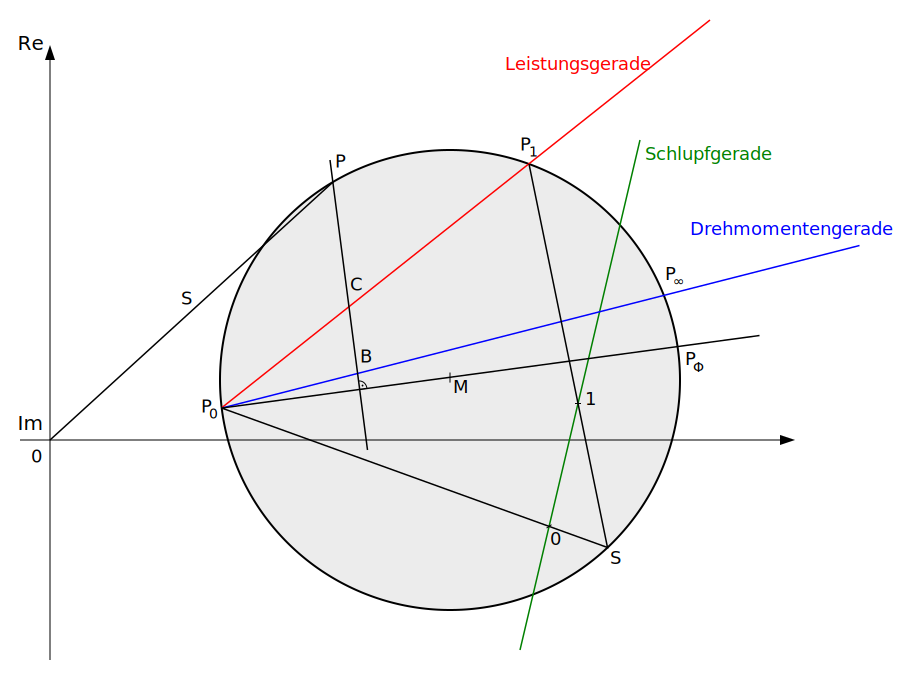
\includegraphics[scale=0.4]{./3_Stand_der_Technik/Abbildungen/Kreisdiagramm_1}
			\caption{Kreisdiagram einer Asynchronmaschine\cite{Wikipedia2024}}
	\end{figure}
	
	
	
	\subsection{Gleichstrommaschine}
	Die Gleichstrommascheine besteht im Stator entweder aus Permanetmagneten, oder aus permanent-erregten Erregerwicklung. Der Rotor besteht aus Wicklungen, welche durch einen Kommutator (auch Stromwender genannt) und B�rsten mithilfe von Gleichspannung versorgt werden. Die Drehzahl der Maschine kann hierbei ganz einfach durch Ver�ndern der Versorgungsspannung linear geregelt werden. 
	
	\begin{figure}[H]
			\centering
			\includegraphics[scale=0.8]{./3_Stand_der_Technik/Abbildungen/Gleichstrommaschine_1}
			\caption{Aufbau Gleichstrommaschine\cite{Pischtschan2024}}
	\end{figure}
	
	Vorteil des Gleichstrommotors ist seine einfach Drehzahlregelung durch Ver�nderung der Spannung, Nachteil der hohe Wartungsaufwand und Verschlei� der Maschine. Er wird aufgrund von sinkenden Preisen bei Frequenzumrichtern immer weniger verwendet.
	
	\input{./3_Stand_der_Technik/7.3_FE_Synchronmaschine}
	
	\input{./3_Stand_der_Technik/7.4_PE_Synchronmaschine}
	
	\input{./3_Stand_der_Technik/7.5_Positionsmessung}
	
	\subsection{Trapezf�rmige Regelung}
%%BLDC Motor wird auch Blockstrommotor genannt
%%evtl noch Schrittmotor inkludieren
	
	\input{./3_Stand_der_Technik/7.7_FOC_Regelung}
	
	\fancyfoot[C]{Sandri}
\section{Spannungsversorgung}

	\subsection{Energiespeicher}
	Das Ziel des Energiespeichers ist es m�glichst viel Energie in einem m�glichst kleinen Volumen zu speichern und diese effizient aufzunehmen und abzugeben. Der Aufbau dieser Batterien besteht meistens aus zwei unterschiedlichen Elektroden und aus einem dazwischen befindlichen Elektrolyt. Die Spannung einer solchen Zelle h�ngt von  der Differenz der Elektronegativit�t der beiden Elektroden ab. Die wichtigsten Eckdaten eines Akkus sind seine Spannung in V, seine Kapazit�t in Wh und die Endlade- und Laderate in C($\frac{Entladestrom}{Kapazit\ddot{a}t}$). Die meisten Akkus bestehen aus mehreren Zellen die in Serie oder parallel geschalten sind, um entweder Spannung oder Kapazit�t zu erh�hen. Daraus entstehen Bezeichnungen f�r Akkus wie zum Beispiel 4S2P, welches f�r 4 Serielle Zellen, 2 mal parllel geschalten steht. 
	
	\begin{figure}[H]
		\centering
		\includegraphics[scale=0.4]{./3_Stand_der_Technik/Abbildungen/Akku_3}
		\caption{Serien- und Parallelschaltung von Akkuzellen\cite{heliplanet.com2024}}
	\end{figure}
	
	Bei Akkus mit mehreren Zellen ist es wichtig darauf zu achten, dass die Zellspannung der unterschiedlichen Zellen nicht variiert. Wenn eine Zelle voll geladen und eine zweite komplett entladen ist, wirkt der Akku anhand der gesamten Akku-Spannung als zur H�lfte geladen. Wenn jedoch eine Entladestrom flie�t, wird eine Zelle unter ihre Abschaltspannung geladen, was zum Schaden der Zelle oder wie im Fall von Lithium Zellen auch zum Brand oder zur Explosion f�hren kann. Um diesem Problem vorzubeugen sind auf Akkus mit mehreren Zellen Balance Stecker angebracht, mithilfe von welchen die einzelnen Zellspannungen gemessen und ausgeglichen werden k�nnen. Der Ausgleich der Zellspannungen findet meistens bei jedem Ladevorgang statt.
	
	\begin{figure}[H]
		\centering
		\includegraphics[scale=0.5]{./3_Stand_der_Technik/Abbildungen/Akku_4}
		\caption{Balance-Stecker\cite{heliplanet.com2024}}
	\end{figure}

	\subsubsection{Alkali-Mangan-Zelle(AlMn)}
		Alkali-Mangan Batterien sind das am h�ufigsten verwendete Batteriesystem, sie �berzeugen vorallem mit ihrer hohen Verf�gbarkeit und g�nstigen Herstellung. Sie bieten auch eine recht hohe Energiedichte. Sie haben auch eine lange Haltbarkeit und ein niedrige Selbstentladung. Zu den Nachteilen z�hlt die geringe Entladerate, die oft unter 0,1C liegt und die begrenzte Wideraufladbarkeit. Die h�ufigste Form dieser Batterie ist die AA und AAA Batterie.\cite{Fricke2007} Die Zellspannung einer Alkali-Mangan-Zelle betr�gt 1,5V.
		
		\begin{figure}[H]
			\centering
			\includegraphics[scale=0.5]{./3_Stand_der_Technik/Abbildungen/Akku_1}
			\caption{Alkali-Mangan-Zelle\cite{Fricke2007}}
		\end{figure}
	
	\subsubsection{Silberoxid-Zelle(AgO)}
		Silberoxid Zellen werden vorwiergend f�r sehr kleine Knopfzellen verwendet, wo hohe Energiedichte ebenso wie geringes Volumen hohe Priorit�t hat. Ihr Aufbau ist sehr �hnlich zu dem der Alkali-Mangan-Zelle. Da die Materialien in gro�en Mengen sehr teuer sind, wird sie meistens nur in geringen Gr��en verwendet. Die Zellspannung einer Silberoxid-Zelle betr�gt 1,6V.\cite{Fricke2007} 
		
		\begin{figure}[H]
			\centering
			\includegraphics[scale=0.5]{./3_Stand_der_Technik/Abbildungen/Akku_2}
			\caption{Silberoxid-Zelle\cite{Fricke2007}}
		\end{figure}
	
	\subsubsection{Nickel-Cadmium-Zelle(NiCd)}
		Nicke-Cadmium-Zellen �berzeugen vorallem durch ihre hohe Belastbarkeit, Schnellladef�higkeit und K�lteresistenz. Sie haben jedoch einen relativ geringen Energieinhalt im Vergleich zu Lithium- oder Alkalisystemen. Ein ebenso gro�er Nachteil is das Auftreten des Memory-Effekts, wenn die Zelle vor dem Vollst�ndig Entladen wieder aufgeladen wird, k�nnen sich Kristalle bilden, die die Kapazit�t wesentlich verringern. Nickel-Cadmium-Zellen haben eine Zellspannung von 1,2V.
	
	\subsubsection{Nickel-Metallhybrid-Zelle(NiMH)}
	
	\subsubsection{Lithium-Ion-Zelle{Li-Ion}}
	
	\subsubsection{Lithium-Polymer-Zelle}
	
	\subsection{Gleichspannungswandler}
	Das Ziel von Gleichspannungswandlern ist es m�glichst verlustarm Gleichspannung entweder hochzuwandeln oder runterzuwandeln. Diese Spannungswandler werden in 3 Kategorien geteilt.
	
	\subsubsection{Tiefsetzsteller(Buck-Converter)}
		Der Tiefsetzsteller funktioniert mithilfe von einem Schalttransistor (meist ein MOSFET) welches mit einem bestimmten Duty-Cycle(Tastgrad) ein- und ausgeschalten wird. Wenn der Schalter geschlossen ist, steigt der Strom durch die Induktivit�t langsam an und es flie�t kein Strom durch die Diode. Wenn der Schalter nun ge�ffnet wird, sinkt der Strom der durch die Diode flie�t, linear ab und der Strom flie�t nun durch
	
	\begin{figure}[H]
		\centering
		\includegraphics[scale=0.2]{./3_Stand_der_Technik/Abbildungen/Spannungswandler_1}
		\caption{Schaltbild eines Tiefsetzstellers\cite{wikipedia2024a}}
	\end{figure}
	
	\subsubsection{Hochsetzsteller(Boost-Converter)}
	
	\subsubsection{Hoch- und Tiefsetzsteller(Buck- and Boost-Converter)}
	
	\newpage
	\newpage
\fancyfoot[C]{Gürel}
\section{Sensorik}
\fancyfoot[C]{G�rel}
\subsection{LiDAR Sensoren}
LiDAR-Sensoren sind ein essenzielles Instrument in der modernen Sensorik, welche erm�glichen, pr�zise Messungen der Umgebungen zu erstellen. 
Die einfachsten Sensoren bestehen aus einem Time-of-Flight (TOF) Distanzmesser, welches einen Lichtpuls sendet und die Zeit misst, die es f�r die R�ckkehr ben�tigt. 
Die LiDAR Sensoren werden grunds�tzlich in 3 Kategorien aufgeteilt:

\paragraph{1D-LiDAR}
In seiner grundlegendsten Form besteht der LiDAR-Sensor aus einem Distanzmesser, der seine Reichweite in einer einzigen Dimension misst. 
Dieser Ansatz erm�glicht eine schnelle Erfassung von Entfernungen entlang einer Linie, was als 1D-LiDAR bekannt ist. 
Die Genauigkeit dieser Messungen h�ngt von verschiedenen Faktoren ab, wie der Leistung des Laserimpulses, der Empfindlichkeit des Photosensors und der Rotationsgeschwindigkeit der Basis. 
Diese Ger�te sind im Handwerk verbreitet und haben bei geringen Kosten eine hohe Genauigkeit.

\paragraph{2D-LiDAR}
Durch die kontinuierliche Rotation des Distanzmessers um eine Achse wird der 1D-LiDAR zu einem 2D-LiDAR erweitert. 
Diese Erweiterung erm�glicht eine Erfassung von Entfernungen entlang einer Linie und gleichzeitig um die eigene Achse herum. 
Dadurch entsteht eine 2D-Karte der Umgebung, die eine detailliertere Darstellung erm�glicht. 
Diese Ger�te sind mechanisch komplex, da der Sensor im Idealen Fall bei exakt gleich bleibender Geschwindigkeit genau horizontal gedreht werden muss. 
Diese Sensoren sind bei autonomen Ger�ten im Indoor-Bereich verbreitet, wie zum Beispiel ein Saug-Roboter oder ein autonomes Lieferfahrzeug in einer Lagerhalle.

\begin{figure}[H]
    \centering
    \includegraphics[scale=0.55]{./3_Stand_der_Technik/Abbildungen/symbolfoto_lidar_C_YDLIDAR.png}
    \caption{Symbolfoto 2D LiDAR Sensor, YDLiDAR G2 \cite{YDLiDAR2024}}
\end{figure}

\paragraph{3D-LiDAR}
Ein weiterer Fortschritt in der LiDAR-Technologie ist der 3D-LiDAR, der nicht nur um eine Achse rotiert, sondern auch in der H�he verstellbar ist. Durch diese zus�tzliche Dimension werden bestimmte H�hen nacheinander abgetastet, wodurch eine vollst�ndige dreidimensionale Punktwolke der Umgebung erstellt wird. Diese Ger�te haben entweder mehrere gestapelte Sensoren um eine Art Punktwolke zu erstellen oder modifizieren die H�he des Lasers von einer einzelnen Quelle. Die Genauigkeit und Aufl�sung dieser Punktwolke h�ngt von der Art des Sensors sowie die Pr�zision und der Rotationsmechanik ab.

\paragraph{Anwendung und Bedeutung}
LiDAR-Sensoren finden in verschiedenen Anwendungen Anwendung, darunter Gel�nde- und Geb�udevermessung sowie Unterst�tzung autonomer Fahrzeuge. Die M�glichkeit, pr�zise Entfernungen zu messen und detaillierte 3D-Karten zu erstellen, macht sie unverzichtbar f�r Projekte, die eine genaue Umgebungswahrnehmung erfordern. Die Erfassung der Intensit�t des reflektierten Lichts erm�glicht zudem eine detaillierte Oberfl�chencharakterisierung, was in vielen Anwendungen von gro�em Nutzen ist.


\fancyfoot[C]{G�rel}
\subsection{Ultraschallsensoren}
Ultraschallsensoren bestehen aus einem Schallwandler und einer Empfangseinheit. Der Schallwandler sendet Ultraschallwellen aus, die an Objekten reflektiert werden und von der Empfangseinheit erfasst werden. 
Tonwellen ab 20 kHz gelten als Ultraschall und k�nnen demnach nicht vom Menschen geh�rt werden, die Sensoren operieren unter diesem Bereich \cite{Frantzen2024}. 
Die Zeitmessung zwischen Aussenden und Empfangen des Schallsignals erm�glicht die Berechnung der Entfernung zum Objekt. 

Ultraschallsensoren bieten eine kosteng�nstige L�sung f�r die Abstandsmessung und werden h�ufig als Fahrzeugparkassistenz oder in der Robotik verwendet. Der generelle Anwendungsbereich ist jener, bei dem eine grobe Ann�herung der Entfernung ausreicht.


\fancyfoot[C]{G�rel}
\subsection{Radar Sensoren}
Radar (Radio Detection and Ranging) Sensoren bestehen aus einer Sendeantenne und einer Empfangsantenne. Die Sendeantenne sendet hochfrequente elektromagnetische Wellen aus, die von Objekten reflektiert werden und von der Empfangsantenne erfasst werden. Die Zeitmessung zwischen Aussenden und Empfangen des Signals erm�glicht die Berechnung der Entfernung zum Objekt. 

Radar bietet eine effektive M�glichkeit, Entfernungen zu messen und Bewegungen zu verfolgen. Es wird h�ufig in der Luft- und Seefahrt, der Wetterbeobachtung, der Verkehrs�berwachung und der milit�rischen Anwendung eingesetzt. Im Vergleich zu LiDAR und Ultraschallsensoren bietet Radar eine gr��ere Reichweite und ist weniger anf�llig f�r Umwelteinfl�sse wie Nebel oder Regen.

	
\subsection{Kameras}
Kameras haben eine entscheidende Rolle in der Personenerkennung und im Bereich der K�nstlichen Intelligenz (KI), insbesondere in Anwendungen wie Video�berwachung, Gesichtserkennung und biometrischer Authentifizierung. Verschiedene Aspekte der Kamera, wie Objektiv, Fokus und Blende, beeinflussen die Leistung und Genauigkeit dieser Anwendungen.

\textbf{Objektiv:} Das Objektiv einer Kamera bestimmt, wie Licht auf den Bildsensor f�llt und beeinflusst somit die Bildqualit�t und Sch�rfe. In Anwendungen der Personenerkennung ist ein hochwertiges Objektiv wichtig, um klare und detaillierte Bilder aufzunehmen. Die Wahl des Objektivs h�ngt von den spezifischen Anforderungen der Anwendung ab, wie zum Beispiel dem Blickwinkel und der Entfernung zum zu erfassenden Objekt.

\textbf{Fokus:} Der Fokus einer Kamera bestimmt, welche Teile eines Bildes scharfgestellt werden und welche unscharf bleiben. In der Personenerkennung ist ein breiter Fokusbereich von entscheidender Bedeutung, um Personen klar und deutlich zu erfassen, unabh�ngig von ihrer Entfernung zur Kamera. Ausserdem kann ein schneller Autofokus es der Kamera erm�glichen, sich schnell an sich bewegende Personen anzupassen und klare Bilder aufzunehmen.

\textbf{Blende:} Die Blende einer Kamera reguliert die Menge an Licht, die auf den Bildsensor f�llt, und beeinflusst somit die Belichtung und Tiefensch�rfe eines Bildes. In Anwendungen der Personenerkennung ist eine angemessene Belichtung entscheidend, um klare und gut sichtbare Bilder zu gew�hrleisten, insbesondere bei unterschiedlichen Lichtverh�ltnissen. Eine variable Blende kann dabei helfen, sich an wechselnde Lichtbedingungen anzupassen und optimale Ergebnisse zu erzielen.

\textbf{Anwendung im KI-Bereich:} Im Bereich der K�nstlichen Intelligenz werden Kameras h�ufig f�r die Erfassung von Trainingsdaten verwendet, um KI-Modelle f�r die Personenerkennung zu trainieren. Hochaufl�sende Bilder, die von Kameras aufgenommen werden, dienen als Eingabe f�r diese Modelle, um Personen zu identifizieren und zu klassifizieren. Die Qualit�t der aufgenommenen Bilder, die durch die oben genannten Faktoren beeinflusst wird, tr�gt wesentlich zur Leistungsf�higkeit und Genauigkeit der KI-Modelle bei.

	
	
	\section{Rechensysteme}

	\fancyfoot[C]{G�rel}
\subsection{Einplatinencomputer}

Ein Einplatinencomputer ist eine kompakte Computerplatine, die alle wichtigen Komponenten eines Computers enth�lt, einschlie�lich Prozessor, Speicher, E/A-Ports und vieles mehr. Diese Computer sind oft kosteng�nstig und vielseitig einsetzbar, was sie f�r eine Vielzahl von Anwendungen attraktiv macht.

\paragraph{Raspberry Pi}

Der Raspberry Pi ist eine Serie von Einplatinencomputern, die alle mit einer ARM Cortex CPU betrieben werden. Die Firma Raspberry Pi ist vor allem in der Hobbyzone f�r ihre kosteng�nstigen und zuverl�ssigen Systeme bekannt. Diese kleinen, aber leistungsstarken Computer bieten eine Vielzahl von Anwendungsm�glichkeiten, von der Heimautomatisierung �ber die Robotik bis hin zur Entwicklung von Prototypen f�r IoT-Ger�te. Sie sind f�r ihre einfache Handhabung und ihre breite Unterst�tzung in der Entwicklergemeinschaft beliebt.

\paragraph{LattePanda}

Der LattePanda ist eine Serie von Einplatinencomputern, die die x86-Architektur mit Intel-CPUs verwenden. Der im Projekt verwendete LattePanda 3 Delta verf�gt �ber zwei M.2-Steckpl�tze (PCIe und SATA), von denen einer mit der Google Coral TPU belegt worden ist. Diese Kombination erm�glicht die Rechenleistung f�r s�mtliche ben�tigten KI-Anwendungen. Der Einsatz von x86-Architektur und Intel-CPUs bietet eine breite Kompatibilit�t mit vorhandener Software und erleichtert die Integration von externen Ger�ten und Erweiterungen. Der LattePanda Delta 3 bietet somit eine leistungsstarke Plattform f�r KI-Anwendungen und andere rechenintensive Projekte.

\paragraph{Nvidia Jetson}

Der Nvidia Jetson ist ein System-on-a-Module (SoM) mit einer NVIDIA Recheneinheit, welche speziell auf KI-Anwendungen ausgerichtet ist. Aufgrund seiner ausgezeichneten Leistungsf�higkeit und seiner speziellen Ausrichtung auf KI-Berechnungen w�re der Jetson f�r das Projekt ideal geeignet. Allerdings sind die Kosten f�r den Jetson vergleichsweise hoch, was ihn als Option ausschlie�t. Der Nvidia Jetson bietet eine solide Leistung f�r KI-Anwendungen, ist jedoch m�glicherweise nicht die kosteng�nstigste Option f�r das Projekt.

Im Vergleich dazu bietet der LattePanda Delta 3 eine kosteng�nstigere Alternative mit den erforderlichen Funktionen f�r das Projekt. Durch die Verwendung von Intel-CPUs und der x86-Architektur erm�glicht der LattePanda Delta 3 dennoch eine solide Leistung f�r KI-Anwendungen. Die Verf�gbarkeit von zwei M.2-Steckpl�tzen, von denen einer mit der Google Coral TPU belegt ist, bietet die erforderliche Rechenleistung f�r die geplanten KI-Anwendungen. Obwohl der LattePanda Delta 3 nicht speziell f�r KI-Anwendungen entwickelt wurde, bietet er dennoch eine kosteng�nstige L�sung mit ausreichender Rechenleistung und Erweiterungsm�glichkeiten f�r das Projekt.

	
	\input{./3_Stand_der_Technik/11.6_Hardwarebeschleunigung.tex}
	
	\fancyfoot[C]{Gürel}
\section{Softwareentwicklung}

	
	\input{./3_Stand_der_Technik/11.1.1_Software_Einleitung.tex}
	
	\input{./3_Stand_der_Technik/11.1.2_Bibliotheken.tex}
	
	\input{./3_Stand_der_Technik/11.1.3_Versionsverwaltung.tex}
	
	\input{./3_Stand_der_Technik/11.1.4_GitHub}
	
	\input{./3_Stand_der_Technik/11.1.5_RRT.tex}
	
	

	
	\fancyfoot[C]{G�rel}
\subsection{Grundlagen ROS}
Das Robot Operating System (ROS) bietet ein flexibles und leistungsstarkes Ger�st f�r die Entwicklung von Software f�r Roboter und andere automatisierte Maschinen oder Anlagen. Es bietet eine Vielzahl von Werkzeugen, Bibliotheken und Konventionen, die Entwicklern dabei helfen, komplexe Anwendungen zu erstellen.

\paragraph{Modularit�t und Wiederverwendbarkeit: }
ROS ist auf Modularit�t ausgelegt, was bedeutet, dass verschiedene Komponenten eines Projekts als unabh�ngige Pakete entwickelt und wiederverwendet werden k�nnen. Dies erm�glicht eine saubere und strukturierte Entwicklung und erleichtert die Wartung und Skalierung von Systemen.

\paragraph{Kommunikation und Nachrichtenaustausch: }
Ein zentrales Konzept in ROS ist die Nachrichtenvermittlung, die es erm�glicht, dass verschiedene Teile eines Robotersystems miteinander kommunizieren k�nnen. ROS verwendet ein Publisher/Subscriber-Modell, bei dem Knoten Nachrichten �ber definierte Themen austauschen k�nnen. Dies erm�glicht eine lose Kopplung zwischen den Komponenten und erleichtert die Integration neuer Funktionen.

\paragraph{Publisher/Subscriber-Modell: }
ROS basiert auf einem Publisher/Subscriber-Modell, bei dem Knoten Nachrichten �ber definierte Themen austauschen k�nnen. Ein Knoten kann Nachrichten auf einem Thema ver�ffentlichen (\textit{publish}), und andere Knoten k�nnen sich auf dieses Thema abonnieren (\textit{subscribe}), um die Nachrichten zu empfangen. Dies erm�glicht eine lose Kopplung zwischen den Komponenten und erleichtert die Integration neuer Funktionen.
\begin{figure}[H]
    \centering
    \includegraphics[scale=0.4]{./3_Stand_der_Technik/Abbildungen/ExchangeDataWithROSPublishersAndSubscribersExample_01.png}
    \caption{Illustration vom Nachrichtenaustausch der Nodes \cite{TheMathWorks2024}}
\end{figure}
\paragraph{Vordefinierte Nachrichtentypen: }
ROS bietet eine Vielzahl von vordefinierten Nachrichtentypen, die h�ufig in der Robotik verwendet werden. Dazu geh�ren Nachrichten wie \textit{LaserScan}, die Informationen �ber Laserabtastungen enthalten, oder \textit{IMU} (Inertial Measurement Unit), die Daten �ber die Orientierung und Bewegung eines Roboters liefern. Diese vordefinierten Nachrichtentypen erm�glichen eine einfache und standardisierte Kommunikation zwischen den verschiedenen Komponenten eines Robotersystems.

\paragraph{Anpassbare Nachrichten: }
Zus�tzlich zu den vordefinierten Nachrichtentypen k�nnen Entwickler auch eigene Nachrichtentypen definieren, um spezifische Anforderungen ihrer Anwendung zu erf�llen. Dies erm�glicht eine hohe Flexibilit�t und Anpassbarkeit bei der Entwicklung von Anwendungen und er�ffnet M�glichkeiten f�r die Integration neuer Sensoren, Aktuatoren und Algorithmen.

	
	\fancyfoot[C]{G�rel}
\subsection{Kartographie Algorithmen}
In ROS stehen verschiedene Algorithmen zur Verf�gung, die es Robotern erm�glichen, ihre Umgebung zu kartieren und eine interne Darstellung der Welt um sie herum zu erstellen. Diese spielen eine entscheidende Rolle bei der Umgebungswahrnehmung und der sicheren Navigation von Robotern.

\paragraph{Hector SLAM}
Hector SLAM \cite{Kohlbrecher2011}ist ein Kartographie Algorithmus in ROS, der auf der Nutzung von Laserscannern basiert. Dieser Algorithmus verwendet eine Sch�tzmethode, um die Position und Orientierung eines Roboters basierend auf den Laserdaten zu bestimmen. Durch kontinuierliches Scannen der Umgebung und die Verfolgung von Merkmalen kann Hector SLAM eine pr�zise Karte der Umgebung erstellen. Ein wesentlicher Vorteil dieses Algorithmus ist seine Effizienz und Robustheit, auch in Umgebungen mit begrenzter Sichtbarkeit oder Bewegungseinschr�nkungen.

\paragraph{Google Cartographer}
Google Cartographer \cite{Hess2016}, ein in ROS integrierter Kartographie Algorithmus, basiert auf dem Prinzip der simultanen Lokalisierung und Kartierung (SLAM), wobei er Laserscanner- und IMU-Daten nutzt, um eine Karte der Umgebung zu generieren. Google Cartographer wird h�ufig in autonomen Fahrzeugen und Robotern eingesetzt, um pr�zise Umgebungskarten zu erstellen. Eine besonders herausragende Eigenschaft des Google Cartographers liegt in seiner Unabh�ngigkeit von Odometriedaten, was ihn besonders attraktiv macht, insbesondere bei diesem Projekt, da solche Daten nicht vollst�ndig verf�gbar sind. Diese Option erweist sich als vorteilhaft und erm�glicht eine zuverl�ssige Kartierung auch unter herausfordernden Bedingungen.
\begin{figure}[H]
    \centering
    \includegraphics[scale=0.165]{./3_Stand_der_Technik/Abbildungen/google_slam_symbolbild.png}
    \caption{Symbolbild einer erstellten Karte vom Cartographer \cite{Hess2016}}
\end{figure}
\paragraph{Anpassung und Integration}
Beide Kartographie Algorithmen bieten M�glichkeiten zur Anpassung und Integration in ROS. Entwickler k�nnen die Parameter der Algorithmen an die spezifischen Anforderungen ihres Projekts anpassen und sie in bestehende Robotikanwendungen integrieren. Dies erm�glicht es, hochpr�zise Karten der Umgebung zu erstellen und sie f�r die Navigation und Steuerung von Robotern zu verwenden.

	
	\fancyfoot[C]{G�rel}
\subsection{KI-Berechnungen}

K�nstliche Intelligenz (KI) basiert auf komplexen mathematischen Modellen und Algorithmen, die es Computern erm�glichen, menschen�hnliche Entscheidungen zu treffen oder Muster in Daten zu erkennen. Viele dieser Algorithmen verwenden Matrixberechnungen als Grundlage f�r ihre Funktionsweise.

\paragraph{Warum sind KI-Berechnungen Matrixberechnungen?}

KI-Algorithmen, insbesondere neuronale Netzwerke, verwenden Matrixoperationen, um Daten zu verarbeiten und Muster zu erkennen. Ein neuronales Netzwerk besteht aus mehreren Schichten von Neuronen, die miteinander verbunden sind. Jedes Neuron nimmt Eingaben von anderen Neuronen entgegen, multipliziert sie mit Gewichtungen und f�hrt eine Aktivierungsfunktion aus, um ein Ergebnis zu erzeugen. Diese Operationen k�nnen effizient in Form von Matrixmultiplikationen durchgef�hrt werden.

In einem neuronalen Netzwerk werden die Gewichtungen zwischen den Neuronen als Gewichtsmatrizen dargestellt. Die Eingaben werden ebenfalls in Form von Matrizen dargestellt. Durch die Anwendung von Matrixoperationen k�nnen komplexe Berechnungen parallelisiert und effizient auf Grafikprozessoren (GPU) oder speziell entwickelten Tensor Processing Units (TPU) durchgef�hrt werden. Durch das Ver�ndern dieser Gewichte wird eine KI �trainiert�, wobei in einer �Generation� mehrere Matrizen miteinander verglichen werden, und die beste Variante als Basis der n�chsten Generation ausgew�hlt wird.

\paragraph{Warum sind TPUs f�r KI-Berechnungen besser geeignet?}

Tensor Processing Units (TPUs) sind speziell f�r die Beschleunigung von KI-Berechnungen optimierte Hardwareeinheiten. Im Gegensatz zu herk�mmlichen CPUs oder GPUs sind TPUs darauf ausgelegt, Matrixoperationen effizient durchzuf�hren, was zu einer erheblichen Beschleunigung von KI-Anwendungen f�hrt.

TPUs sind in der Lage, gro�e Datenmengen schnell zu verarbeiten und komplexe neuronale Netzwerke in Echtzeit zu trainieren. Ihre Architektur ist darauf ausgerichtet, die spezifischen Anforderungen von KI-Anwendungen zu erf�llen.

\paragraph{Aufbau neuronaler Netze als Matrix}

Neuronale Netzwerke werden oft als Matrizen von Gewichtungen und Eingaben dargestellt. Jedes Neuron in einem neuronalen Netzwerk kann als Knoten in einer Schicht betrachtet werden, wobei die Verbindungen zwischen den Neuronen als Gewichtungsmatrizen repr�sentiert werden. Durch die Kombination von Matrixmultiplikationen und Aktivierungsfunktionen k�nnen neuronale Netzwerke komplexe Berechnungen durchf�hren und Muster in Daten erkennen.

	
	\fancyfoot[C]{G�rel}
\subsection{Einplatinencomputer}

Ein Einplatinencomputer ist eine kompakte Computerplatine, die alle wichtigen Komponenten eines Computers enth�lt, einschlie�lich Prozessor, Speicher, E/A-Ports und vieles mehr. Diese Computer sind oft kosteng�nstig und vielseitig einsetzbar, was sie f�r eine Vielzahl von Anwendungen attraktiv macht.

\paragraph{Raspberry Pi}

Der Raspberry Pi ist eine Serie von Einplatinencomputern, die alle mit einer ARM Cortex CPU betrieben werden. Die Firma Raspberry Pi ist vor allem in der Hobbyzone f�r ihre kosteng�nstigen und zuverl�ssigen Systeme bekannt. Diese kleinen, aber leistungsstarken Computer bieten eine Vielzahl von Anwendungsm�glichkeiten, von der Heimautomatisierung �ber die Robotik bis hin zur Entwicklung von Prototypen f�r IoT-Ger�te. Sie sind f�r ihre einfache Handhabung und ihre breite Unterst�tzung in der Entwicklergemeinschaft beliebt.

\paragraph{LattePanda}

Der LattePanda ist eine Serie von Einplatinencomputern, die die x86-Architektur mit Intel-CPUs verwenden. Der im Projekt verwendete LattePanda 3 Delta verf�gt �ber zwei M.2-Steckpl�tze (PCIe und SATA), von denen einer mit der Google Coral TPU belegt worden ist. Diese Kombination erm�glicht die Rechenleistung f�r s�mtliche ben�tigten KI-Anwendungen. Der Einsatz von x86-Architektur und Intel-CPUs bietet eine breite Kompatibilit�t mit vorhandener Software und erleichtert die Integration von externen Ger�ten und Erweiterungen. Der LattePanda Delta 3 bietet somit eine leistungsstarke Plattform f�r KI-Anwendungen und andere rechenintensive Projekte.

\paragraph{Nvidia Jetson}

Der Nvidia Jetson ist ein System-on-a-Module (SoM) mit einer NVIDIA Recheneinheit, welche speziell auf KI-Anwendungen ausgerichtet ist. Aufgrund seiner ausgezeichneten Leistungsf�higkeit und seiner speziellen Ausrichtung auf KI-Berechnungen w�re der Jetson f�r das Projekt ideal geeignet. Allerdings sind die Kosten f�r den Jetson vergleichsweise hoch, was ihn als Option ausschlie�t. Der Nvidia Jetson bietet eine solide Leistung f�r KI-Anwendungen, ist jedoch m�glicherweise nicht die kosteng�nstigste Option f�r das Projekt.

Im Vergleich dazu bietet der LattePanda Delta 3 eine kosteng�nstigere Alternative mit den erforderlichen Funktionen f�r das Projekt. Durch die Verwendung von Intel-CPUs und der x86-Architektur erm�glicht der LattePanda Delta 3 dennoch eine solide Leistung f�r KI-Anwendungen. Die Verf�gbarkeit von zwei M.2-Steckpl�tzen, von denen einer mit der Google Coral TPU belegt ist, bietet die erforderliche Rechenleistung f�r die geplanten KI-Anwendungen. Obwohl der LattePanda Delta 3 nicht speziell f�r KI-Anwendungen entwickelt wurde, bietet er dennoch eine kosteng�nstige L�sung mit ausreichender Rechenleistung und Erweiterungsm�glichkeiten f�r das Projekt.

	
	\input{./3_Stand_der_Technik/11.6_Hardwarebeschleunigung.tex}

%% Mechanik %%%%%%%%%%%%%%%%%%%%%%%%%%%%%%%%%%%%%%%%%%%%%%%%%
\newpage
\chapter{Mechanik}
	\fancyfoot[C]{Kaltenleitner}
	\section{Mechanischer Aufbau}

	Bei dem mechanischen Aufbau von Athena sind viele Faktoren zu beachten. Ein paar dieser Faktoren w�ren der Verwendungszweck, Kosten und die Belastbarkeit. Ebenfalls gibt es auch Modellautos, welche ihre Funktion und Stabilit�t schon am Markt bewiesen haben. Da alle bereits existierenden Fahrzeuge die hohen platztechnischen Anspr�che eines solchen Projekts nicht vollst�ndig erf�llen, ist es besser, das Fahrzeug von Grund auf selbst zu konstruieren. Ein Fahrzeug mit hoher Karosserie ist von Vorteil, da ein solches viel Platz bietet.\\
\\
	F�r den mechanischen Aufbau stehen viele Materialien mit unterschiedlichen Eigenschaften und Preisen zur Verf�gung. Auch kann man sich an Teilen von bereits vorhandenen Fahrzeugen bedienen. Dies wurde im Falle von Athena auch getan. So werden mehrere Teile aufgrund der hohen Kosten im Falle der Eigenanfertigung vom etablierten Modell "X-MAXX" der Firma Traxxas genutzt. Diese Teile umfassen die Lager, D�mpfer und gro�e Teile des Antriebsstrangs. Aufgrund der �bernommenen Komponenten hat man einen gewissen Rahmen, in dem sich bei der Auslegung der Gesamtgr��e bewegen muss. Die Bauteile, die hierbei am meisten ausmachen, sind die Grundplatte und die zentrale Antriebswelle.

\subsection{Grundlegender Aufbau / Montagereihenfolge}
\subsubsection{Antriebsstrang}
	Beim Zusammenbau von Athena wird der Antriebsstrang als erstes montiert. Seine Hauptaufgabe besteht darin, die Leistung vom Motor auf die Reifen zu �bertragen. Der Allradantrieb setzt sich aus drei Differenzialen zusammen. Bei der Konstruktion m�ssen die Abst�nde zwischen dem Kegelrad (gro�es Zahnrad des Differentials) und dem Ritzel ber�cksichtigt werden. Wenn diese nicht passen, kann dies dazu f�hren, dass die Zahnr�der bei hoher Belastung leichter besch�digt werden. Es ist wichtig, beim Zusammenbau auf die Schmierung des Getriebes und der Differenziale zu achten.
		
		\begin{figure}[H]
			\centering
			\includegraphics[scale=2.4]{./4_Mechanik/Abbildungen/Aufbau_Anleitung_render/Antriebsstrang_1}
			\caption{ Antriebsstrang ohne obere Getriebegeh�use}
		\end{figure}

%% Elektronik %%%%%%%%%%%%%%%%%%%%%%%%%%%%%%%%%%%%%%%%%%%%%%%
\newpage
\chapter{Elektronik}
	
	\fancyfoot[C]{Sandri}
\section{Spannungsversorgung}

	\subsection{Wahl der Akkus}
		Bei der Wahl der Akkus sind einige Faktoren zu beachten:
		
		\begin{itemize}
		
			\item Die Entladerate des Akkus muss hoch genug sein, um den Motor


	
	\input{./5_Elektronik/2_Computer}
	
	\input{./5_Elektronik/3_Hauptplatine}
	
	\input{./5_Elektronik/4_Motor}

%% Software %%%%%%%%%%%%%%%%%%%%%%%%%%%%%%%%%%%%%%%%%%%%%%%%%
\newpage
\chapter{Software}
	
	\fancyfoot[C]{Sandri}
\section{Programmierung des ESP32-Mikrocontrollers}
	Die Aufgaben des ESP32 bestehen aus dem Auslesen aller Sensordaten, dem Steuern der Beleuchtung und der Kommunikation mit dem Bordcomputer. Da der ESP32 2 Kerne besitzt wird der Code zwischen diesen aufgeteilt, das Einlesen aller Sensoren und die Kommunikation l�uft auf Kern 0, das Programm f�r die Beleuchtung auf Kern 1. Um den beiden Kernen getrennt Aufgaben zuordnen zu k�nnen, m�ssen im void Setup() 2 Tasks, welche an einen bestimmten Kern gebunden sind, erstellt werden.
	
	\lstset{style=VS2017}
	\begin{lstlisting}[language=C, caption={ESP32 2 Kerne Setup}]
void setup() {

	Serial.begin(115200);

	xTaskCreatePinnedToCore(
				Task1setup,   /* Task function. */
				"Task1",     /* name of task. */
				10000,       /* Stack size of task */
				NULL,        /* parameter of the task */
				1,           /* priority of the task */
				&Task1,      /* Task handle to keep track of created task */
				0);          /* pin task to core 0 */                  
	delay(500); 

	xTaskCreatePinnedToCore(
				Task2setup,   /* Task function. */
				"Task2",     /* name of task. */
				10000,       /* Stack size of task */
				NULL,        /* parameter of the task */
				1,           /* priority of the task */
				&Task2,      /* Task handle to keep track of created task */
				1);          /* pin task to core 1 */
	delay(500);

}
	\end{lstlisting}
	

	\subsection{Kern 0 / Sensoren und Kommunikation}
	Die Hauptaufgabe von Kern 0 ist es, mit dem Bordcomputer zu kommuniziern, alle Sensordaten auszulesen, und Komponenten, wie zum Beispiel L�fter, zu steuern.
	Die Seriellen Schnittstellen vom ESP32 und dem Bordcomputer sind mithilfe des Shields verbunden, um eine fl�ssige Kommunikation zu gew�hrleisten, ist ein Protokoll n�tig:
	
	\subsubsection{Aufbau von Paketen zwischen ESP32 und Bordcomputer}
		Der grunds�tzliche Aufbau eines Paktes zwischen ESP32 und Bordcomputer ist immer gleich, er besteht aus folgenden Teilen
			
			\begin{enumerate}
			
				\item Datentyp: LED, Temp, Volt, IMU1, IMU2, Sonar, FAN, Error //Alle m�glichen Daten, die zwischen ESP und Bordcomputer gesendet werden k�nnen. 
				
				\item Anzahl der Datenwerte
				
				\item Access, Read / Write / Both  //Sollen die Daten nur eingelesen werden, wird nur eine Antwort erwartet oder wird beides erwartet?
				
				\item Daten, je nach Anzahl der Datenwerte k�nnen hier beliebig viele Werte hintereinander geschrieben werden
				
				\item Error, wird ein Fehler gemeldet?
			
			\end{enumerate}
			
			Jedes Datenpaket beginnt mit einem Marker und endet mit einem Marker, in diesem Fall wurde als StartMarker "x" verwendet und als EndMarker "y". Die Daten sind in dazwischen in genannter Reihenfolge mit Beistrichen getrennt.
			Die Gr��e der verschiedenen Datenpaktet ist wiefolgt:
			
			\begin{table}[H]
				\centering
				\caption{Datenpakete}
				
				\begin{tabular}{|c|c|c|c|c|c|}
					
					\hline
					\multicolumn{6}{|c|}{\textbf{Datenpakete}}\\
					\hline
					\hline
					\textbf{Name} & \textbf{Datentyp} & \textbf{Anzahl der Variablen} & \textbf{Access} & \textbf{Daten} & \textbf{Error} \\
					\hline
					IMU1 & 1 & 6 & 1 & - & 0 \\
					\hline
					IMU2 & 2 & 3 & 1 & - & 0 \\
					\hline
					OctoSonar & 3 & 16 & 1 & - & 0 \\
					\hline
					Spannungssensoren & 4 & 5 & 1 & - & 0 \\
					\hline
					Temperatursensoren & 5 & 6 & 1 & - & 0 \\
					\hline
					L�fter & 6 & 4 & 2 & - & 0 \\
					\hline
					LEDs & 7 & 4 & 2 & - & 0 \\
					\hline
					IsOK & 0 & 0 & 2 & - & 0 \\
					\hline
					
				\end{tabular}
			\end{table}
			
			Access = 0 bedeutet, dass Daten nur vom ESP gelesen werden und es keine Antwort gibt.\\
			Access = 1 bedeutet, dass Daten an den Bordcomputer vom ESP geschickt werden sollen.\\
			Access = 2 bedeutet, dass Daten vom ESP eingelesen werden sollen und dass eine Antwort geschickt werden soll.\\
			\\
			Error = 0 bedeutet, das kein Fehler vorhanden ist.\\
			Error = 1 bedeutet, dass eine Warnung vorhanden ist.\\
			Error = 2 bedeutet, dass ein fataler Fehler vorhanden ist.\\
			
		\subsubsection{Einlesen der Pakete am ESP32}
			F�r die Kommunikation zwischen ESP32 und Bordcomputer ist eine eigene Bibliothek verantwortlich, so muss im Hauptprogramm nur eine Objekt "Computer" erstellt werden, um Daten einzulesen beziehungsweise zu empfangen.
			Die erste Funktion der Bilbiothek lie�t die Daten ein und speichert sie in einem Buffer:
			
			\lstset{style=VS2017}
			\begin{lstlisting}[language=C, caption={Einlesen eines Pakets}]
bool LattePandacomms::refresh(char startMarker, char endMarker) {
  
  _inProgress = false;
  
  while (Serial.available() > 0) {    //Checks for Serial Data
    
    byte x = Serial.read();   //Reads Serial Data
    
    if (x == startMarker && _inProgress == false) {    //IF the first Byte = startMarker, start to recieve Data
       
      _bytesRecvd = 0;      //Zero bytes have been recieved so far
      _inProgress = true;   //New Message has started
      
      for(int i = 0; i < sizeof(BufferIn); i++) {   //Clear BufferIn Array to make space for new message
        BufferIn[i] = '\0';
      }
      
    }
    
    if (_inProgress ) {   //Has the message started?
          
      if (_bytesRecvd<_maxMessage) {    //Does the current length exceed the max Message limit
        
        BufferIn[_bytesRecvd++] = x;  //Save current Byte to Buffer
        
      }
      
      if (x == endMarker) {     //End of message 
        
        _inProgress = false;    //Reset inprogress variable
        //allReceived = true;
        _nb = _bytesRecvd;
        return 1;
        
      }
      
    }

    
  }
  
  //Serial.println(BufferIn);   //DEBUG
  return 0;
  
}			
			\end{lstlisting}
			
			Diese Funktion wartet auf den StartMarker und speichert anschlie�end bis zum Erscheinen des EndMarkers jede Ziffer in ein Buffer-Array, welches danach weiterverarbeitet werden kann.
			
			\subsubsection{Dekodieren der Pakete am ESP32}
					Um das sich im Buffer befindliche Paket nun zu dekodieren sind zwei zus�tzliche Funktionen n�tig:\\
					Die Erste Funktion entfernt den Start-und Endmarker, da diese nicht dekodiert werden m�ssen.\\
					Mithilfe von der zweiten Funktion ist m�glich den ersten Wert aus einem Char-Array zu l�schen. So kann nun immer der erste Wert eingelesen werden und dann gel�scht werden. Dies wird so oft widerholt, bis die gew�nschte Anzahl an Variablen(durch Anzahl der Variablen im Paket gegeben) eingelesen ist.\\
					Diese eingelesen Variablen werden in Komponenten, die durch ein struct definiert sind, im public Teil der Class abgespeichert, so ist es m�glich vom Hauptcode auf diese zuzugreifen:
					
					\lstset{style=VS2017}
					\begin{lstlisting}[language=C, caption={Datenspeicherort und Struktur}]
struct Component {    //Struktur des Datenspeicherorts
  uint8_t Type;
  uint8_t nVal;
  uint8_t Access;
  uint8_t Data[maxnDataVar];
  uint8_t Error;
};

class LattePandacomms {
public:
  
  LattePandacomms();

  Component IsOk;
  Component IMU1;
  Component IMU2;
  Component Octosonar;
  Component Voltage;
  Component Temp;
  Component Fan;
  Component LED;
}						
					\end{lstlisting}
					
			\subsubsection{}		
	
	\subsection{Kern 1 / Beleuchtung}

	
	\section{LattePanda} %%Titel nix fix bitte �ndern wenn n�tig
	
	\section{Benutzeroberfl�che} %%Titel nix fix bitte �ndern wenn n�tig

%% K�nstliche Intelligenz %%%%%%%%%%%%%%%%%%%%%%%%%%%%%%%%%%%
\newpage
\chapter{Anwendung k�nstlicher Intelligenz}
	TEST

%% Ergebnisse %%%%%%%%%%%%%%%%%%%%%%%%%%%%%%%%%%%%%%%%%%%%%%%
\newpage
\fancyfoot[C]{Sandri, Kaltenleitner, G�rel, Petrovic}
\chapter{Ergebnisse und Ausblick}

Das Projekt hat bedeutende Fortschritte gemacht, wobei verschiedene Teams erfolgreich an ihren jeweiligen Aufgaben gearbeitet haben. Die Teamleitung und Entwicklung des elektronischen Aufbaus, einschlie�lich des Kabelbaums und des Antriebssystems, wurden erfolgreich abgeschlossen. Ebenso wurde die Softwareentwicklung f�r den Mikrocontroller sowie der 3D-Druck der Bauteile erfolgreich durchgef�hrt.

Die Finanzierung des Projekts wurde abgeschlossen, und die Benutzeroberfl�chen sowie das Webdesign wurden erstellt und m�ssen nun integriert werden. Der mechanische Aufbau, das Design und der Aufbau des Antriebsstrangs, der Aufh�ngung, der Lenkung und der Karosserie wurden erfolgreich fertiggestellt, ebenso wie die Fertigung und der Zusammenbau der mechanischen Bauteile.

Bez�glich der Herausforderungen gab es Probleme mit der Spannungsversorgung aufgrund qualitativ minderwertiger Komponenten, was wiederholt zu Defekten an Sensoren f�hrte. Lieferzeiten und Bestelldauern einiger Komponenten stellten ebenfalls Hindernisse dar. Ein Kurzschluss auf der Platine war ebenfalls ein Problem, das angegangen werden musste.

F�r die Zukunft steht die Fertigstellung der Integration von Finanzierung, Benutzeroberfl�chen und Webdesign sowie die Entwicklung des ROS-Systems und die Umsetzung von Pathfinding, Personenerkennung und Steuerung des Fahrzeugs an. Mit diesen Schritten werden wir das Projekt abschlie�en und die gesteckten Ziele erreichen.




%%%%%%%%%%%%%%%%%%%%%%%%%%%%%%%%%%%%%%%%%%%%%%%%%%%%%%%%%%%%%
%% LITERATUR UND ANDERE VERZEICHNISSE
%%%%%%%%%%%%%%%%%%%%%%%%%%%%%%%%%%%%%%%%%%%%%%%%%%%%%%%%%%%%%
\newpage
%% Ein kleiner Abstand zu den Kapiteln im Inhaltsverzeichnis (toc)
\addtocontents{toc}{\protect\vspace*{\baselineskip}}

%%%%%%%%%%%%%%%%%%%%%%%%%%%%%%%%%%%%%%%%%%%%%%%%%%%%%%%%%%%%%
%% LITERATUR UND ANDERE VERZEICHNISSE
%%%%%%%%%%%%%%%%%%%%%%%%%%%%%%%%%%%%%%%%%%%%%%%%%%%%%%%%%%%%%
%% Ein kleiner Abstand zu den Kapiteln im Inhaltsverzeichnis (toc)
\addtocontents{toc}{\protect\vspace*{\baselineskip}}

%% Literaturverzeichnis
\bibliographystyle{plain}
\bibliography{literatur}


%% Abbildungsverzeichnis
\clearpage
\addcontentsline{toc}{chapter}{Abbildungsverzeichnis}
\listoffigures

%% Tabellenverzeichnis
\clearpage
\addcontentsline{toc}{chapter}{Tabellenverzeichnis}
\listoftables



%%%%%%%%%%%%%%%%%%%%%%%%%%%%%%%%%%%%%%%%%%%%%%%%%%%%%%%%%%%%%
%% ANH�NGE
%%%%%%%%%%%%%%%%%%%%%%%%%%%%%%%%%%%%%%%%%%%%%%%%%%%%%%%%%%%%%
\appendix
%% ==> Schreiben Sie hier Ihren Text oder f�gen Sie externe Dateien ein.

%\input{Dateiname} %Eine Datei 'Dateiname.tex' wird hierf�r ben�tigt.

\chapter{Anhang}

	\section{Stromlaufpl�ne}
\includepdf[pages=-,angle=0]{./9_Anhang/Stromlaufplaene/Shield_0.pdf}
	
	\section{Bema�ungen}
\includepdf[pages=-,angle=0]{./9_Anhang/Bemassung/Bemassungen.pdf}
	
	%%%%%%%%%%%%%%%%%%%%%%%%%%%%%%%%%%%%%%%
\lstset{
   backgroundcolor=\color{white},
	 commentstyle=\color{blue},
 	 keywordstyle=\color{magenta},
   extendedchars=true,
   basicstyle=\footnotesize\ttfamily,
   showstringspaces=false,
   showspaces=false,
   numbers=left,
   numberstyle=\footnotesize,
   numbersep=9pt,
   tabsize=2,
   breaklines=true,
   showtabs=false,
   captionpos=b
}
\begin{lstlisting} [language=HTML,caption={HTML-Code Landing Page}]
<!DOCTYPE html> 
<html lang="en"> 
<head> 
    <meta charset="UTF-8"> <!-- Deklaration der Zeichenkodierung --> 
    <meta name="viewport" content="width=device-width, initial-scale=1.0"> <!-- Viewport-Einstellungen f�r responsive Darstellung auf verschiedenen Ger�ten --> 
    <title>ATHENA</title> <!-- Titel der Webseite --> 
    <link rel="stylesheet" href="https://cdnjs.cloudflare.com/ajax/libs/font-awesome/6.0.0-beta3/css/all.min.css"> <!-- Einbindung von Font Awesome f�r Symbole --> 
    <link rel="stylesheet" href="style.css"> <!-- Einbindung von externem CSS-Stylesheet --> 
    <link href="https://fonts.googleapis.com/css2?family=Orbitron:wght@400;500&display=swap" rel="stylesheet"> <!-- Einbindung von Google Fonts --> 
    <link href="https://fonts.googleapis.com/css2?family=Ethnocentric&display=swap" rel="stylesheet"> <!-- Einbindung von Google Fonts --> 
</head> 
<body> 
 
<section class="header"> <!-- Header-Bereich der Webseite --> 
    <nav> <!-- Navigationsleiste --> 
        <a href="http://www.htl-salzburg.ac.at/startseite.html"><img src="images/HTLlogo.png"> </a> <!-- Link zum Startseite-Bild --> 
        <div class="nav-links" id="nav-links"> <!-- Navigationslinks --> 
            <i class="fa-solid fa-xmark" onclick="hideMenu()"></i> <!-- Schlie�en-Symbol mit Klickfunktion --> 
            <ul> <!-- Ungeordnete Liste f�r Navigationslinks --> 
                <li><a href="">HOME</a></li> <!-- Navigationslink "HOME" --> 
                <li><a href="https://www.instagram.com/projectrccar?igsh=eWhpb2Jtem1wemZt">INSTAGRAM</a></li><!-- Navigationslink "INSTAGRAM" --> 
                <li><a href="https://www.instagram.com/htl.salzburg?igsh=MzFreDNpaWs5bXp2">HTL-Salzburg</a></li><!-- Navigationslink "HTL-Salzburg" --> 
            </ul> 
        </div> 
        <i class="fa-solid fa-bars" onclick="showMenu()"></i> <!-- Burgermen�-Symbol mit Klickfunktion --> 
    </nav> 
 
    <div class="text-box"> <!-- Textbox im Header --> 
        <h1>ATHENA</h1> <!-- �berschrift "ATHENA" --> 
        <a href="INTERACT.html" class="hero-btn">INTERACT</a> <!-- Button mit Verweis auf "INTERACT.html" --> 
    </div> 
</section> 
 
<section class="project"> <!-- Bereich f�r das Projekt --> 
    <h2>Project RC-Car</h2> <!-- �berschrift "Project RC-Car" --> 
    <p>Teile des Projektes</p> <!-- Textabschnitt zur Beschreibung des Projektes --> 
 
    <div class="row"> <!-- Zeile f�r Kurs-Sektionen --> 
        <div class="course-col"> <!-- Spalte f�r den Kurs "Elektronik" --> 
            <h3>Elektronik</h3> <!-- �berschrift "Elektronik" --> 
            <a href="elektronik.html" class="elektronik">Elektronik</a> <!-- Verweis auf "elektronik.html" mit Klassenattribut "elektronik" --> 
        </div> 
 
        <div class="course-col"> <!-- Spalte f�r den Kurs "Mechanik" --> 
            <h3>Mechanik</h3> <!-- �berschrift "Mechanik" --> 
            <a href="mechanik.html" class="mechanik">Mechanik</a> <!-- Verweis auf "mechanik.html" mit Klassenattribut "mechanik" --> 
        </div> 
 
        <div class="course-col"> <!-- Spalte f�r den Kurs "Software" --> 
            <h3>Software</h3> <!-- �berschrift "Software" --> 
            <a href="software.html" class="software">Software</a> <!-- Verweis auf "software.html" mit Klassenattribut "software" --> 
        </div> 
    </div> 
</section> 
 
<section class="about"> <!-- Bereich f�r Informationen �ber das Team --> 
    <h1>Unser Team</h1> <!-- �berschrift "Unser Team" --> 
    <p>Philipp Kaltenleitner, Mert G&uuml;rel, Felix Sandri, David Petrovic</p> <!-- Namen der Teammitglieder --> 
    <div class="einleitung"> <!-- Einleitungstext --> 
        <h5>Einleitung</h5> <!-- �berschrift "Einleitung" --> 
        <p>Willkommen auf der Website unseres Diplomarbeitsprojekts "Athena" an der HTLBLuVA Salzburg, Elektrotechnik-Abteilung!<br> <!-- Einleitungstext --> 
            Seit vier Jahren arbeiten wir leidenschaftlich an der Entwicklung eines selbstfahrenden Modellautos. Als Sch�ler der Elektrotechnik haben wir an der HTLBLuVA Salzburg ein umfassendes Verst�ndnis f�r innovative Technologien erworben.<br> <!-- Einleitungstext --> 
            Unser Projekt "Athena" vereint Elektrotechnik, Programmierung und Robotik, um ein fortschrittliches autonomes Modellauto zu schaffen. Durch intensive Forschung und technologische Innovationen gestalten wir die Zukunft der Mobilit&auml;t mit. <br> <!-- Einleitungstext --> 
            Erforschen Sie auf dieser Website unsere Reise, Entwicklungen und Erfolge. "Athena" repr&auml;sentiert nicht nur unsere Leidenschaft f�r Elektrotechnik, sondern auch unseren Beitrag zur Evolution autonomer Fahrzeuge.<br> <!-- Einleitungstext --> 
            Vielen Dank f�r Ihr Interesse. Begleiten Sie uns auf unserer Reise durch Innovation und Elektrotechnik. 
        </p> 
    </div> 
</section> 
\end{lstlisting}

%%%%%%%%%%%%%%%%%%%%%%%%%%%%%%%%%%%%%%%%%%%%%%%

\begin{lstlisting} [language=CSS,caption={CSS-Code Landing Page}]
/* Globale Stile f�r alle Elemente */ 
* { 
    margin: 0; /* Setzt den Au�enabstand auf 0, um unerw�nschte Leerzeichen zu vermeiden */ 
    padding: 0; /* Setzt das Innenpolster auf 0, um unerw�nschte Leerzeichen zu vermeiden */ 
    font-family: 'Orbitron', sans-serif; /* Verwendet die Schriftart Orbitron f�r den gesamten Text */ 
} 
 
/* Stile f�r die Ueberschriftsklasse */ 
.title { 
    font-family: 'Ethnocentric', sans-serif; /* Verwendet die Schriftart Ethnocentric f�r Elemente mit der Klasse 'title' */ 
} 
 
/* Stile f�r den Header-Bereich */ 
.header { 
    min-height: 100vh; /* Setzt die Mindesthoehe auf 100% der Bildschirmh�he */ 
    width: 100%; /* Setzt die Breite auf 100% */ 
    background-image: linear-gradient(rgba(4,9,30,0.7),rgba(4,9,30,0.7)),url(images/RC_Car.jpeg); /* Verwendet ein lineares Farbverlaufshintergrundbild */ 
    background-position: center; /* Zentriert das Hintergrundbild */ 
    background-size: cover; /* Skaliert das Hintergrundbild, um den gesamten Container zu bedecken */ 
    position: relative; /* Setzt die Position auf relativ, um absolute Positionierung innerhalb des Headers zu ermoeglichen */ 
} 
 
/* Stile f�r die Navigationsleiste */ 
nav { 
    display: flex; /* Verwendet Flexbox f�r das Layout */ 
    padding: 2% 6%; /* F�gt Innenpolster hinzu */ 
    justify-content: space-between; /* Platzierung der Elemente mit gleichem Abstand dazwischen */ 
    align-items: center; /* Zentriert die Elemente vertikal */ 
} 
 
/* Stile f�r das Logo in der Navigationsleiste */ 
nav img { 
    width: 150px; /* Festgelegte Breite des Logos */ 
    position: absolute; /* Absolute Positionierung f�r die Positionierung innerhalb des Headers */ 
    top: 10px; /* Abstand vom oberen Rand */ 
    left: 15px; /* Abstand vom linken Rand */ 
} 
 
/* Stile f�r die Navigationslinks */ 
.nav-links { 
    flex: 1; /* Nimmt verf�gbaren Platz ein */ 
    text-align: right; /* Ausrichtung der Links nach rechts */ 
} 
 
/* Stile f�r die Navigationslinksliste */ 
.nav-links ul li { 
    list-style: none; /* Entfernt die Standardlistenformatierung */ 
    display: inline-block; /* Platzierung der Links nebeneinander */ 
    padding: 8px 12px; /* Innenpolster f�r die Links */ 
    position: relative; /* Positionierung f�r den Hover-Effekt */ 
} 
 
/* Stile f�r die Navigationslink-Texte */ 
.nav-links ul li a { 
    color: black; /* Textfarbe */ 
    text-decoration: none; /* Entfernt die Unterstreichung der Links */ 
    font-size: 15px; /* Schriftgroe�e */ 
} 
 
/* Stile f�r den Hover-Effekt der Navigationslinks */ 
.nav-links ul li::after { 
    content: ''; /* Fuegt ein Pseudo-Element hinzu */ 
    width: 0%; /* Breite auf 0 setzen */ 
    height: 2px; /* H�he des Balkens */ 
    background: #f44336; /* Hintergrundfarbe des Balkens */ 
    display: block; /* Blockelement */ 
    margin: auto; /* Zentriert den Balken horizontal */ 
    transition: 0.5s; /* Animations�bergang */ 
} 
 
/* Stile f�r den Hover-Effekt der Navigationslinks */ 
.nav-links ul li:hover::after { 
    width: 100%; /* Breite des Balkens auf 100% setzen */ 
} 
 
/* Stile f�r die Textbox im Header */ 
.text-box { 
    width: 90%; /* Breite der Textbox */ 
    color: #000000; /* Textfarbe */ 
    position: absolute; /* Absolute Positionierung innerhalb des Headers */ 
    top: 50%; /* Positionierung in der Mitte vertikal */ 
    left: 50%; /* Positionierung in der Mitte horizontal */ 
    transform: translate(-50%,-50%); /* Zentrierung der Textbox */ 
    text-align: center; /* Zentrierung des Textes */ 
} 
 
/* Stile f�r die �berschrift in der Textbox */ 
.text-box h1 { 
    font-size: 60px; /* Schriftgroe�e */ 
} 
 
/* Stile f�r den Text in der Textbox */ 
.text-box p { 
    margin: 10px 0 40px; /* Au�enabstand */ 
    font-size: 14px; /* Schriftgroe�e */ 
    color: #fff; /* Textfarbe */ 
} 
 
/* Stile f�r den Hero-Button */ 
.hero-btn { 
    display: inline-block; /* Inline-Block-Element */ 
    text-decoration: none; /* Entfernt die Unterstreichung */ 
    color: #fff; /* Textfarbe */ 
    border: 1px solid #fff; /* Randstil */ 
    padding: 12px 34px; /* Innenpolster */ 
    font-size: 13px; /* Schriftgroe�e */ 
    background: transparent; /* Transparenter Hintergrund */ 
    position: relative; /* Positionierung */ 
    cursor: pointer; /* Zeigercursor */ 
} 
/* Stile f�r den Hover-Effekt des Hero-Buttons */ 
.hero-btn:hover {border: 1px solid #000000; /* Randfarbe �ndern */ 
    background: #ff3434; /* Hintergrundfarbe aendern */ 
    transition: 1s; /* Animationsuebergang */ 
} 
 
/* Stile f�r das Hamburger-Menue und das Schlie�en-Symbol */ 
nav .fa-bars, 
nav .fa-xmark { 
    display: none; /* Standardmae�ig ausgeblendet */ 
    color: #fff; /* Symbolfarbe */ 
    margin: 10px; /* Au�enabstand */ 
    font-size: 22px; /* Symbolgroe�e */ 
    cursor: pointer; /* Zeigercursor */ 
} 
 
/* Media Query f�r die kleinere Bildschirmgroe�e */ 
@media (max-width: 700px) { 
    .text-box h1 { 
        font-size: 20px; /* Reduzierte Schriftgroe�e f�r kleine Bildschirme */ 
    } 
    .nav-links ul li { 
        display: block; /* Aendert die Anzeige der Navigationslinks auf Block */ 
    } 
    .nav-links { 
        position: absolute; /* Absolute Positionierung f�r das Hamburger-Menue */ 
        background: #f44336; /* Hintergrundfarbe */ 
        height: 100vh; /* Volle Bildschirmhoehe */ 
        width: 200px; /* Breite */ 
        top: 0; /* Positionierung oben */ 
        right: -200px; /* Startposition au�erhalb des Bildschirms */ 
        text-align: left; /* Links ausgerichtet */ 
        z-index: 2; /* Stacking-Kontext */ 
        transition: 1s; /* Animations�bergang */ 
    } 
    nav .fa { 
        display: block; /* Symbol anzeigen */ 
        color: #fff; /* Symbolfarbe */ 
        margin: 10px; /* Au�enabstand */ 
        font-size: 22px; /* Symbolgroe�e */ 
        cursor: pointer; /* Zeigercursor */ 
    } 
    nav .fa-xmark { 
        display: none; /* Schlie�en-Symbol standardmae�ig ausblenden */ 
    } 
    .nav-links ul { 
        padding: 30px; /* Innenpolster f�r die Navigationslinks */ 
    } 
} 
 
/* Stile f�r den Projektabschnitt */ 
.project { 
    width: 80%; /* Breite des Abschnitts */ 
    margin: auto; /* Zentrierung */ 
    text-align: center; /* Zentrierung des Textes */ 
    padding: 30px; /* Innenpolster */ 
} 
 
/* Stile f�r die Zeilen in dem Projektabschnitt */ 
.row { 
    margin-top: 5%; /* Oberer Au�enabstand */ 
    display: flex; /* Flexbox-Layout */ 
    justify-content: space-between; /* Platzierung der Elemente mit gleichem Abstand dazwischen */ 
} 
 
/* Stile f�r die Kurskolonnen */ 
.course-col { 
    flex-basis: 31%; /* Flexbasis */ 
    background: #fff3f3; /* Hintergrundfarbe */ 
    border-radius: 10px; /* Randradius */ 
    margin-bottom: 5%; /* Unterer Au�enabstand */ 
    padding: 20px 12px; /* Innenpolster */ 
    box-sizing: border-box; /* Box-Sizing */ 
    transition: 0.5s; /* Animations�bergang */ 
} 
 
/* Stile f�r die Ueberschriften der Kurskolonnen */ 
h3 { 
    text-align: center; /* Zentrierte Ausrichtung */ 
    font-weight: 600; /* Fettdruck */ 
    margin: 10px 0; /* Au�enabstand */ 
} 
 
/* Stile f�r den Hover-Effekt der Kurskolonnen */ 
.course-col:hover { 
    box-shadow: 0 0 20px 0px rgba(0,0,0,0.2); /* Schatten hinzuf�gen */ 
} 
 
/* Media Query f�r die kleinere Bildschirmgr��e */ 
@media(max-width: 700px) { 
    .row { 
        flex-direction: column; /* �ndert die Flexrichtung auf Spalte */ 
    } 
} 
 
/* Stile f�r den Abschnitt "�ber uns" */ 
.about { 
    width: 80%; /* Breite des Abschnitts */ 
    margin: auto; /* Zentrierung */ 
    text-align: center; /* Zentrierung des Textes */ 
    padding-top: 30px; /* Oberer Innenabstand */ 
} 
 
/* Stile f�r den allgemeinen Text */ 
p { 
    color: #000000; /* Textfarbe */ 
    font-size: 14px; /* Schriftgroe�e */ 
    font-weight: 300; /* Schriftgewicht */ 
    line-height: 22px; /* Zeilenhoehe */ 
    padding: 10px; /* Innenpolster */ 
} 
 
/* Stile f�r den Footer */ 
.footer { 
    position: absolute; /* Absolute Positionierung */ 
    left: 50%; /* Positionierung in der Mitte horizontal */ 
    transform: translateX(-50%); /* Zentrierung */ 
    text-align: center; /* Zentrierung des Textes */ 
} 
 
/* Stile f�r die �berschrift im Footer */ 
.footer h4 { 
    margin-bottom: 10px; /* Unterer Au�enabstand */ 
    margin-top: 20px; /* Oberer Au�enabstand */ 
    font-weight: 600; /* Fettdruck */ 
    color: #333; /* Textfarbe */ 
    font-size: 18px; /* Schriftgroe�e */ 
} 
 
/* Stile f�r die Social-Media-Icons im Footer */ 
.icons .fa-instagram { 
    color: #f44336; /* Icon-Farbe */ 
    margin: 0 20px; /* Au�enabstand */ 
    cursor: pointer; /* Zeigercursor */ 
    font-size: 30px; /* Symbolgroe�e */ 
    padding-top: 20px 0; /* Padding f�r die vertikale Ausrichtung */ 
    padding-bottom: 15px; /* Padding f�r die vertikale Ausrichtung */ 
} 
\end{lstlisting}

HTML-Code Interaktion-Page:
\begin{lstlisting} [language=HTML,caption={HTML-Code Interaktion-Page}]
<!DOCTYPE html>
<html lang="en">
<head>
   <!-- Metadaten -->
   <meta charset="UTF-8"> <!-- Zeichencodierung -->
   <meta name="viewport" content="width=device-width, initial-scale=1.0"> <!-- Viewport-Einstellungen -->
   <title>INTERACT</title> <!-- Titel der Webseite -->
 
   <!-- Einbindung von externen Stylesheets -->
   <link rel="stylesheet" href="https://cdnjs.cloudflare.com/ajax/libs/font-awesome/6.0.0-beta3/css/all.min.css"> <!-- FontAwesome-Bibliothek -->
   <link rel="stylesheet" href="batterie.css"> <!-- Eigene CSS-Datei f�r die Batterien -->
   <link rel="stylesheet" href="style-test.css"> <!-- Eigene CSS-Datei f�r allgemeine Stildefinitionen -->
   <link rel="stylesheet" type="text/css" href="thermo.css"> <!-- Eigene CSS-Datei f�r das Thermometer -->
   <link rel="stylesheet" href="speedo.css"> <!-- Eigene CSS-Datei f�r das Geschwindigkeitsmessger�t -->
   <link rel="preconnect" href="https://fonts.googleapis.com"> <!-- Vorabverbindung zu Google Fonts -->
   <link rel="preconnect" href="https://fonts.gstatic.com" crossorigin> <!-- Vorabverbindung zu Google Fonts -->
   <link href="https://fonts.googleapis.com/css2?family=Orbitron:wght@400;500&display=swap" rel="stylesheet"> <!-- Google Fonts Schriftart "Orbitron" -->
   <link rel="stylesheet" href="https://cdn.jsdelivr.net/npm/@fortawesome/fontawesome-free@6.4.2/css/fontawesome.min.css" integrity="sha384-BY+fdrpOd3gfeRvTSMT+VUZmA728cfF9Z2G42xpaRkUGu2i3DyzpTURDo5A6CaLK" crossorigin="anonymous"> <!-- FontAwesome-Bibliothek (Version 6.4.2) von einem CDN -->
 
</head>
<body>
   <!-- Header-Bereich -->
   <section class="Inter-header">
       <nav>
           <a href="http://www.htl-salzburg.ac.at/startseite.html"><img src="images/HTLlogo.png"></a> <!-- Navigationslink mit dem HTL-Logo -->
       </nav>
       <h1>Interaktion</h1> <!-- �berschrift "Interaktion" -->
       <div class="semi_arc e6"> <!-- Bereich f�r eine Halbkreis-Animation -->
           <div class="semi_arc_3 e5_1">
               <div class="semi_arc_3 e5_2">
                   <div class="semi_arc_3 e5_3">
                       <div class="semi_arc_3 e5_4"></div>
                   </div>
               </div>
           </div>
       </div>
   </section>
 
  <!-- Geschwindigkeitsmessger�t -->
<section class="speedometer"> <!-- Abschnitt f�r das Geschwindigkeitsmessger�t -->
   <div id="el" data-value="0"> <!-- Element f�r das Messger�t -->
       <span id="needle"></span> <!-- Zeiger des Messger�ts -->
   </div>
</section>
 
  
   <!-- Batterien -->
   <section class="batterie bat-1">
       <div class="container">
           <div class="bat-name">Bat-1</div> <!-- Name der Batterie "Bat-1" -->
           <i class="fas fa-3x fa-battery-full icon"></i> <!-- FontAwesome-Symbol f�r volle Batterie -->
           <div class="progress2 progress-moved">
               <div class="progress-bar2"></div> <!-- Fortschrittsleiste f�r die Batterie -->
               <div class="loader" style="--n: 1; --f: 0;"></div> <!-- Ladebalken f�r die Batterie -->
           </div>
       </div>
   </section>
  
   <section class="batterie bat-2">
       <div class="container">
           <div class="bat-name">Bat-2</div> <!-- Name der Batterie "Bat-2" -->
           <i class="fas fa-3x fa-battery-full icon"></i> <!-- FontAwesome-Symbol f�r volle Batterie -->
           <div class="progress2 progress-moved">
               <div class="progress-bar2"></div> <!-- Fortschrittsleiste f�r die Batterie -->
               <div class="loader" style="--n: 1; --f: 0;"></div> <!-- Ladebalken f�r die Batterie -->
           </div>
       </div>
   </section>
  
   <section class="batterie bat-3">
       <div class="container">
           <div class="bat-name">Bat-3</div> <!-- Name der Batterie "Bat-3" -->
           <i class="fas fa-3x fa-battery-full icon"></i> <!-- FontAwesome-Symbol f�r volle Batterie -->
           <div class="progress2 progress-moved">
               <div class="progress-bar2"></div> <!-- Fortschrittsleiste f�r die Batterie -->
               <div class="loader" style="--n: 1; --f: 0;"></div> <!-- Ladebalken f�r die Batterie -->
           </div>
       </div>
   </section>
  
   <section class="batterie bat-4">
       <div class="container">
           <div class="bat-name">Bat-4</div> <!-- Name der Batterie "Bat-4" -->
           <i class="fas fa-3x fa-battery-full icon"></i> <!-- FontAwesome-Symbol f�r volle Batterie -->
           <div class="progress2 progress-moved">
               <div class="progress-bar2"></div> <!-- Fortschrittsleiste f�r die Batterie -->
               <div class="loader" style="--n: 1; --f: 0;"></div> <!-- Ladebalken f�r die Batterie -->
           </div>
       </div>
   </section>
 
   <section class="batterie bat-5">
       <div class="container">
           <div class="bat-name">Batterie</div> <!-- Name der Batterie "Batterie" -->
           <i class="fas fa-3x fa-battery-full icon"></i> <!-- FontAwesome-Symbol f�r volle Batterie -->
           <div class="progress2 progress-moved">
               <div class="progress-bar2"></div> <!-- Fortschrittsleiste f�r die Batterie -->
               <div class="loader" style="--n: 1; --f: 0;"></div> <!-- Ladebalken f�r die Batterie -->
           </div>
       </div>
   </section>
  
 
   <!-- Ihr JavaScript-Inhalt -->
   <script type="text/javascript" src="https://cdnjs.cloudflare.com/ajax/libs/d3/3.4.2/d3.js"></script> <!-- Einbindung von D3.js-Bibliothek -->
   <script type="text/javascript" src="thermo.js"></script> <!-- JavaScript-Datei f�r das Thermometer -->
   <script src="batterie.js"></script> <!-- JavaScript-Datei f�r die Batterien -->
   <script src="speedo.js"></script> <!-- JavaScript-Datei f�r das Geschwindigkeitsmessger�t -->
 
  
</body>
</html>
\end{lstlisting}

%%%%%%%%%%%%%%%%%%%%%%%%%%%%%%%%%%%%

\begin{lstlisting} [language=JavaScript,caption={JavaScript-Code Temperaturanzeige}]
// Diese Funktion wird aufgerufen, wenn das Fenster geladen ist.
window.onload = function initialize() {
   // Erzeugt die Messger�te-Pfade
   createPaths();
   // Startet die Aktualisierung der Messger�te im Intervall von 2000 Millisekunden (2 Sekunden)
   setInterval(updateGauges, 2000);
};
 
// Ein leeres Array zur Speicherung der Messger�te
var gauges = [];
 
// Ein JSON-Objekt mit Beispiel-Temperaturdaten
var jsonTemp = {
   "t1": { "temp": 80.45, "peak": 90 }
};
 
// Funktion zum Erstellen eines Messger�ts mit den angegebenen Parametern
function createGauge(name, label, min, max, sizebias, gx, gy) {
   // Konfigurationsobjekt f�r das Messger�t
   var config = {
       size: 200 + sizebias,
       label: label,
       min: undefined !== min ? min : 0,
       max: undefined !== max ? max : 100,
       coorx: gx,
       coory: gy
   };
 
   // Berechnet den Wertebereich des Messger�ts
   var range = config.max - config.min;
 
   // Erstellt ein neues Messger�t und rendert es
   gauges[name] = new Gauge(name + "GaugeContainer", config);
   gauges[name].render();
}
 
// Funktion zum Erstellen der Pfade f�r die Positionierung der Messger�te
function createPaths() {
   // Positioniert das Messger�t "t1" auf der linken Seite
   createGauge("t1", "T1", 5, 100, 0, 100, 200);
   // Positioniert das Messger�t "t2" auf der rechten Seite
   createGauge("t2", "T2", 30, 100, 0, window.innerWidth - 300, 220);
}
 
// Funktion zum Aktualisieren der Messger�te
function updateGauges() {
   // Durchl�uft alle Messger�te im Array
   for (var key in gauges) {
       // Generiert einen zuf�lligen Wert f�r das Messger�t
       var value = getRandomValue(gauges[key]);
       // Aktualisiert das Messger�t mit dem neuen Wert
       gauges[key].redraw(value);
   }
}
 
// Funktion zum Generieren eines zuf�lligen Werts f�r ein Messger�t
function getRandomValue(gauge) {
   var overflow = 0; //10;
   return Math.floor(gauge.config.min - overflow + (gauge.config.max - gauge.config.min + overflow * 2) * Math.random());
}
 
// Konstruktor f�r ein Messger�t
function Gauge(placeholderName, configuration) {
   // Speichert den Namen des Platzhalters f�r das Messger�t
   this.placeholderName = placeholderName;
   var self = this;
 
   // Konstante f�r Pi
   var pi = 2 * Math.PI;
 
   // String f�r das Gradzeichen
   var degreeString = "00B0";
   var degreeSign = String.fromCharCode(parseInt(degreeString, 16));
 
   // Standardfarbe f�r das Messger�t
   var defaultColor = "#ff5f24";
   var newColor,
       hold;
 
   // Methode zur Konfiguration des Messger�ts
   this.configure = function (configuration) {
       this.config = configuration;
 
       // Festlegen der Gr��e, Mindest- und Maximalwerte und anderer Konfigurationseigenschaften
       this.config.size = this.config.size;
       this.config.min = undefined !== configuration.min ? configuration.min : 0;
       this.config.max = undefined !== configuration.max ? configuration.max : 100;
       this.config.transitionDuration = configuration.transitionDuration || 500;
       this.config.gaugetype = configuration.gaugetype;
       this.config.coorx = configuration.coorx;
       this.config.coory = configuration.coory;
       this.config.cx = this.config.size / 2;
       this.config.cy = this.config.size / 2;
       this.config.inner = this.config.size / (25 / 7);
       this.config.outer = this.config.size / (25 / 9.5);
   };
 
   // Methode zum Rendern des Messger�ts
   this.render = function () {
       // Funktion zum Erstellen eines Bogen-Generators f�r das Messger�t
       var arc = d3.svg.arc()
           .innerRadius(this.config.inner)
           .outerRadius(this.config.outer)
           .startAngle(0);
 
       // Erstellt das Container-Div f�r das Messger�t
       this.container = d3.select("body")
           .append("div")
           .attr("id", this.config.label + "Temp")
           .attr("class", "tempContainer")
           .style("left", this.config.coorx + "px")
           .style("top", this.config.coory + "px")
           .style("position", "absolute");
 
       // Erstellt das SVG-Element f�r das Messger�t
       this.body = this.container
           .append("svg")
           .attr("width", this.config.size)
           .attr("height", this.config.size);
 
       // Erstellt Filterdefinitionen f�r visuelle Effekte
       var defs = this.body.append("defs");
       var filter = defs.append("filter")
           .attr("id", "drop-shadow")
           .attr("height", "130%");
       filter.append("feGaussianBlur")
           .attr("in", "SourceAlpha")
           .attr("stdDeviation", 2)
           .attr("result", "blur");
       filter.append("feOffset")
           .attr("in", "blur")
           .attr("dx", 0)
           .attr("dy", 0)
           .attr("result", "offsetBlur");
       var feMerge = filter.append("feMerge");
       feMerge.append("feMergeNode")
           .attr("in", "offsetBlur");
       feMerge.append("feMergeNode")
           .attr("in", "SourceGraphic");
 
       // Erstellt einen Container f�r den Zeiger des Messger�ts
       var pointerContainer = this.body.append("g")
           .attr("class", "pointerContainer")
           .attr("transform", "translate(" + this.config.size / 2 + "," + this.config.size / 2 + ")")
           .style("position", "absolute");
 
       // Erstellt den Hintergrund des Messger�ts
       pointerContainer
           .append("path")
           .datum({ endAngle: pi })
           .style("fill", "#565656")
           .attr("d", arc);
       // Erstellt den Vordergrund des Messger�ts
       pointerContainer
           .append("path")
           .datum({ endAngle: this.valueToRadians(this.config.min) })
           .style("fill", "#ff5f24")
           .attr("class", "foreground")
           .attr("d", arc);
 
       // Erstellt den K�rper des Messger�ts
       pointerContainer
           .append("circle")
           .style("fill", "#e6e7e8")
           .style("class", "gaugebody")
           .style("filter", "url(#drop-shadow)")
           .attr("r", this.config.inner);
 
       // Berechnet den mittleren Wert des Messger�ts
       var midValue = (this.config.min + this.config.max) / 2;
 
       // Berechnet die Schriftgr��e basierend auf der Gr��e des Messger�ts
       var fontSize = Math.round(this.config.size / 15);
 
       // F�gt den Text f�r die aktuelle Temperatur hinzu
       pointerContainer
           .append("text")
           .attr("x", this.config.cx - (this.config.cx * 1.0))
           .attr("y", this.config.cy - (this.config.cy * 1.20))
           .attr("text-anchor", "middle")
           .attr("fill", "#58585b")
           .style("font-size", fontSize + "px")
           .text('Current Temp.');
 
       // Aktualisiert die Schriftgr��e f�r den aktuellen Temperaturwert
       fontSize = Math.round(this.config.size / 3.5);
       var current = pointerContainer
           .append("text")
           .attr("x", this.config.cx - (this.config.cx * 0.92))
           .attr("y", this.config.cy - (this.config.cy * 0.7))
           .attr("class", "current")
           .attr("text-anchor", "middle")
           .attr("fill", "#58585b")
           .style("font-size", fontSize + "px")
           .text(this.config.min + degreeSign);
 
       // Ruft die redraw-Methode auf, um das Messger�t zu aktualisieren
       this.redraw(this.config.min, 0);
   };
 
   // Methode zum Aktualisieren des Messger�ts
   this.redraw = function (value, transitionDuration) {
       // Konvertiert den Wert in Grad und Bogenma�
       var degreeValue = this.valueToDegrees(value);
       var pointerValue = this.valueToRadians(value);
       redrawSize = this.config.size;
 
       // Bogen-Generator f�r das Messger�t
       var arc = d3.svg.arc()
           .innerRadius(this.config.inner)
           .outerRadius(this.config.outer)
           .startAngle(0);
 
       // Bestimmt die Farbe des Messger�ts basierend auf dem Wert
       switch (true) {
           case (degreeValue >= 270):
               // Dunkelrot
               newColor = '#990000';
               break;
           case (degreeValue >= 180):
               // Hellblau
               newColor = '#ff5f24';
               break;
           case (degreeValue >= 90):
               // Hellrot
               newColor = '#009eff';
               break;
           default:
               // Dunkelblau
               newColor = '#065aa9';
               break;
       }
 
       // Aktualisiert den Text f�r die aktuelle Temperatur
       var current = this.body.select(".pointerContainer");
       current.select(".current")
           .transition()
           .text(value + degreeSign);
 
       // Aktualisiert die Farbe des Vordergrunds des Messger�ts mit �bergang
       foreground = this.body.select(".pointerContainer");
       foreground.select(".foreground")
           .transition()
           .duration(750)
           .styleTween("fill", function () {
               return d3.interpolate(newColor, defaultColor);
           })
           .call(arcTween, pointerValue);
 
       // Speichert die Standardfarbe
       hold = defaultColor;
       defaultColor = newColor;
       newColor = hold;
 
       // Funktion f�r die �bergangsberechnung des Bogens
       function arcTween(transition, newAngle) {
           transition.attrTween("d", function (d) {
               var interpolate = d3.interpolate(d.endAngle, newAngle);
               return function (t) {
                   d.endAngle = interpolate(t);
                   return arc(d);
               };
           });
       }
   };
 
   // Methode zur Umrechnung eines Werts in Grad
   this.valueToDegrees = function (value) {
       return Math.floor(value / this.config.max * 360);
   };
 
   // Methode zur Umrechnung eines Werts in Bogenma�
   this.valueToRadians = function (value) {
       return this.valueToDegrees(value) * Math.PI / 180;
   };
 
   // Konfiguriert das Messger�t
   this.configure(configuration);
}
\end{lstlisting}

%%%%%%%%%%%%%%%%%%%%%%%%%%%%%%%%%%%%%%%%%%%%%%%%%%%%%%%%%%%%%%%%%%%%

\begin{lstlisting} [language=JavaScript,caption={Batterie.js-Code Akkustand}]
CSS.registerProperty({
   name: "--p",
   syntax: "<integer>",
   initialValue: 0,
   inherits: true,
 });
\end{lstlisting}

Speedo.js:
\begin{lstlisting} [language=JavaScript,caption={Speedo.js-Code Speedometer}]
// Elemente mit den entsprechenden IDs aus dem DOM abrufen
var needle = document.getElementById('needle'); // Das zu messende Element
var el = document.getElementById('el'); // Das Element, auf dem der gemessene Winkel als Datenattribut gesetzt wird
 
// Funktion zur Messung der Rotation des Elements 'needle' und Aktualisierung des Winkels im Datenattribut des Elements 'el'
var measureDeg = function() {
 // Die Rotation des Elements 'needle' �ber die CSS-Transformationseigenschaft abrufen
 var st = window.getComputedStyle(needle, null);
 var tr = st.getPropertyValue("-webkit-transform") ||
          st.getPropertyValue("-moz-transform") ||
          st.getPropertyValue("-ms-transform") ||
          st.getPropertyValue("-o-transform") ||
          st.getPropertyValue("transform") ||
          "fail...";
 
 // Die Transformationsmatrix in einzelne Werte aufteilen
 var values = tr.split('(')[1];
     values = values.split(')')[0];
     values = values.split(',');
 var a = values[0];
 var b = values[1];
 var c = values[2];
 var d = values[3];
 
 // Die Skalierung des Elements 'needle' berechnen
 var scale = Math.sqrt(a*a + b*b);
 
 // Den Winkel der Rotation berechnen und in Grad umrechnen
 var sin = b/scale;
 var angle = Math.round(Math.atan2(b, a) * (180/Math.PI));
 
 // Den berechneten Winkel als Datenattribut 'data-value' auf das Element 'el' setzen
 el.setAttribute('data-value', angle);
};
 
// Die Funktion 'measureDeg' in regelm��igen Abst�nden alle 10 Millisekunden aufrufen, um die Rotation des Elements 'needle' fortlaufend zu messen
var periodicalID = setInterval(measureDeg, 10);
\end{lstlisting}

style-test.css:
\begin{lstlisting} [language=CSS,caption={Style-test.css-Code Interaktion-Page}]
/* Globale Stile */
* {
   margin: 0; /* Alle Seitenr�nder auf 0 setzen */
   padding: 0; /* Alle Polster auf 0 setzen */
   font-family: 'Orbitron', sans-serif; /* Standardschriftart f�r alle Elemente festlegen */
}
 
/* Titelstil */
.title {
   font-family: 'Ethnocentric', sans-serif; /* Spezifische Schriftart f�r Elemente mit der Klasse "title" festlegen */
}
 
/* Header-Stil */
.header {
   min-height: 100vh; /* Mindesth�he des Headers auf 100% der Bildschirmh�he setzen */
   width: 100%; /* Volle Breite des Headers */
   background-image: linear-gradient(rgba(4,9,30,0.7),rgba(4,9,30,0.7)),url(images/RC_Car.jpeg); /* Hintergrundbild mit Verlauf und Bild */
   background-position: center; /* Hintergrundbild zentrieren */
   background-size: cover; /* Hintergrundbild anpassen */
   position: relative; /* Position relativ f�r die Positionierung von Kindelementen festlegen */
}
 
/* Navigationsmen�stil */
nav {
   display: flex; /* Flexibles Layout f�r das Navigationsmen� festlegen */
   padding: 2% 6%; /* Innenabstand oben und unten 2%, links und rechts 6% */
   justify-content: space-between; /* Elemente im Navigationsmen� gleichm��ig verteilen */
   align-items: center; /* Elemente vertikal zentrieren */
}
 
nav img {
   width: 150px; /* Breite des Navigationsmen�-Logos */
   position: absolute; /* Absolute Positionierung f�r das Logo */
   top: 10px; /* Abstand vom oberen Rand */
   left: 15px; /* Abstand vom linken Rand */
}
 
/* Stil der Navigationslinks */
.nav-links {
   flex: 1; /* Flexibles Wachstum f�r den mittleren Bereich des Navigationsmen�s */
   text-align: right; /* Text rechts ausrichten */
}
 
.nav-links ul li {
   list-style: none; /* Listenpunkte entfernen */
   display: inline-block; /* Elemente nebeneinander anzeigen */
   padding: 8px 12px; /* Innenabstand oben und unten 8px, links und rechts 12px */
   position: relative; /* Relative Positionierung f�r untergeordnete Elemente */
}
 
.nav-links ul li a {
   color: black; /* Textfarbe der Navigationslinks */
   text-decoration: none; /* Unterstreichung der Links entfernen */
   font-size: 15px; /* Schriftgr��e der Links */
}
 
.nav-links ul li::after {
   content: ''; /* Inhalt hinzuf�gen */
   width: 0%; /* Breite auf 0% setzen */
   height: 2px; /* H�he des Unterstrichs */
   background: #f44336; /* Hintergrundfarbe des Unterstrichs */
   display: block; /* Als Blockelement anzeigen */
   margin: auto; /* Automatische Marge */
   transition: 0.5s; /* �bergangseffekt f�r den Unterstrich */
}
 
.nav-links ul li:hover::after {
   width: 100%; /* Breite des Unterstrichs auf 100% setzen, wenn der Link gehovered wird */
}
 
/* Textfeldstil */
.text-box {
   width: 90%; /* Breite des Textfelds */
   color: #000000; /* Textfarbe */
   position: absolute; /* Absolute Positionierung */
   top: 50%; /* 50% von oben */
   left: 50%; /* 50% von links */
   transform: translate(-50%,-50%); /* Zentrierung des Textfelds */
   text-align: center; /* Text zentrieren */
}
 
.text-box h1 {
   font-size: 60px; /* Schriftgr��e der �berschrift */
}
 
.text-box p {
   margin: 10px 0 40px; /* Au�enabstand oben 10px, unten 40px */
   font-size: 14px; /* Schriftgr��e des Absatzes */
   color: #fff; /* Textfarbe */
}
 
/* Helden-Schaltfl�chenstil */
.hero-btn {
   display: inline-block; /* Als Inline-Blockelement anzeigen */
   text-decoration: none; /* Unterstreichung entfernen */
   color: #fff; /* Textfarbe */
   border: 1px solid #fff; /* Randstil */
   padding: 12px 34px; /* Innenabstand oben und unten 12px, links und rechts 34px */
   font-size: 13px; /* Schriftgr��e */
   background: transparent; /* Transparenter Hintergrund */
   position: relative; /* Relative Positionierung */
   cursor: pointer; /* Zeiger als Cursor */
}
 
.hero-btn:hover {
   border: 1px solid #000000; /* Randstil beim Hover-Effekt */
   background: #ff3434; /* Hintergrundfarbe beim Hover-Effekt */
   transition: 1s; /* �bergangseffekt */
}
 
/* Men�symbolstil */
nav .fa-bars,
nav .fa-xmark {
   display: none; /* Anzeigen des Men�symbols */
   color: #fff; /* Farbe des Symbols */
   margin: 10px; /* Au�enabstand */
   font-size: 22px; /* Symbolgr��e */
   cursor: pointer; /* Zeiger als Cursor */
}
 
@media (max-width: 700px) {
   /* Media Query f�r Bildschirme mit maximaler Breite von 700px */
   .text-box h1 {
       font-size: 20px; /* Schriftgr��e der �berschrift verringern */
   }
   .nav-links ul li {
       display: block; /* Links als Blockelemente anzeigen */
   }
   .nav-links {
       position: absolute; /* Absolute Positionierung des Navigationsmen�s */
       background: #f44336; /* Hintergrundfarbe des Men�s */
       height: 100vh; /* H�he des Men�s auf 100% der Bildschirmh�he setzen */
       width: 200px; /* Breite des Men�s */
       top: 0; /* Abstand vom oberen Rand */
       right: -200px; /* Position vom rechten Rand */
       text-align: left; /* Text linksb�ndig ausrichten */
       z-index: 2; /* Z-Index festlegen */
       transition: 1s; /* �bergangseffekt */
   }nav .fa {
       display: block; /* Anzeigen des Font Awesome-Symbols */
       color: #fff; /* Farbe des Symbols */
       margin: 10px; /* Au�enabstand */
       font-size: 22px; /* Schriftgr��e des Symbols */
       cursor: pointer; /* Zeiger bei Hover */
   }
  
   /* Stil f�r das Schlie�en-Symbol im Navigationsmen� */
   nav .fa-xmark {
       display: none; /* Ausblenden des X-Symbols */
   }
  
   /* Stil f�r die UL-Liste innerhalb des Navigationsmen�s */
   .nav-links ul {
       padding: 30px; /* Innenabstand oben/unten 30px */
   }
  
   /* Projekt-Stile */
   .project {
       width: 80%; /* Breite auf 80% des Elternelements festlegen */
       margin: auto; /* Zentrierung des Elements */
       text-align: center; /* Text zentrieren */
       padding: 30px; /* Innenabstand oben/unten 30px */
   }
  
   /* Stile f�r die Reihe innerhalb des Projekts */
   .row {
       margin-top: 5%; /* Au�enabstand oben 5% */
       display: flex; /* Anzeigen als Flexbox */
       justify-content: space-between; /* Verteilung der Elemente entlang der Hauptachse */
   }
  
   /* Stile f�r die Kurs-Spalten */
   .course-col {
       flex-basis: 31%; /* Basisgr��e der Flexbox */
       background: #fff3f3; /* Hintergrundfarbe */
       border-radius: 10px; /* Abrundung der Ecken */
       margin-bottom: 5%; /* Au�enabstand unten 5% */
       padding: 20px 12px; /* Innenabstand oben/unten 20px, links/rechts 12px */
       box-sizing: border-box; /* Box-Modell: Padding und Border innerhalb der Breite */
       transition: 0.5s; /* �bergangseffekt */
   }
  
   /* �berschriften */
   h3 {
       text-align: center; /* Text zentrieren */
       font-weight: 600; /* Fettschrift */
       margin: 10px 0; /* Au�enabstand oben/unten 10px */
   }
  
   /* Hover-Effekt f�r die Kurs-Spalten */
   .course-col:hover {
       box-shadow: 0 0 20px 0px rgba(0,0,0,0.2); /* Schatten-Effekt */
   }
  
   /* Media Query f�r Bildschirme kleiner als 700px */
   @media(max-width: 700px) {
       .row {
           flex-direction: column; /* �ndern der Flexbox-Richtung auf Spalten */
       }
   }
  
   /* Stile f�r die Projektteile */
   .elektronik,
   .mechanik,
   .software {
       display: inline-block; /* Anzeigen als Inline-Block */
       text-decoration: none; /* Keine Textdekoration */
       color: #000000; /* Textfarbe */
       border: 1px solid #000000; /* Rahmen */
       padding: 10px 30px; /* Innenabstand oben/unten 10px, links/rechts 30px */
       font-size: 13px; /* Schriftgr��e */
       background: transparent; /* Transparenter Hintergrund */
       position: relative; /* Position relativ */
       cursor: pointer; /* Zeiger bei Hover */
   }
  
   /* Hover-Effekt f�r die Projektteile */
   .elektronik:hover,
   .mechanik:hover,
   .software:hover {
       border: 1px solid #000000; /* Rahmenfarbe bei Hover */
       background: #ff3434; /* Hintergrundfarbe bei Hover */
       transition: 1s; /* �bergangseffekt */
   }
  
   /* Stile f�r den Abschnitt �ber uns */
   .about {
       width: 80%; /* Breite auf 80% des Elternelements festlegen */
       margin: auto; /* Zentrierung des Elements */
       text-align: center; /* Text zentrieren */
       padding-top: 30px; /* Innenabstand oben 30px */
   }
  
   /* Textstil f�r den Abschnitt �ber uns */
   p {
       color: #000000; /* Textfarbe */
       font-size: 14px; /* Schriftgr��e */
       font-weight: 300; /* Schriftgewicht */
       line-height: 22px; /* Zeilenh�he */
       padding: 10px; /* Innenabstand */
   }
  
   /* Stile f�r die Einleitung im Abschnitt �ber uns */
   .einleitung {
       width: 60%; /* Breite auf 60% des Elternelements festlegen */
       margin: auto; /* Zentrierung des Elements */
       text-align: center; /* Text zentrieren */
   }
/*-------footer-------*/
.footer {
   position: fixed; /* Positionierung als fest (bleibt am unteren Rand des Bildschirms) */
   bottom: 0; /* Positionierung am unteren Rand */
   left: 0; /* Positionierung am linken Rand */
   width: 100%; /* 100% Breite des Footers */
   background-color: #333; /* Hintergrundfarbe des Footers */
   color: #fff; /* Textfarbe des Footers */
   padding: 20px 0; /* Innenabstand oben und unten */
   text-align: center; /* Zentrieren des Inhalts horizontal */
}
 
.footer h4 {
   margin-bottom: 10px;
   margin-top: 20px;
   font-weight: 600;
   font-size: 18px;
}
 
.icons {
   z-index: 9999; /* Stellen Sie sicher, dass es �ber anderen Elementen liegt */
}
 
.icons .fa-instagram {
   color: #f44336;
   margin: 0 20px;
   cursor: pointer;
   font-size: 30px;
}
 
/*----elektronik--------*/
.elektro-header {
   height: 100vh;
   width: 100%;
   background-image: linear-gradient(rgba(4,9,30,0.7),rgba(4,9,30,0.7)),url(images/Elektronik.jpeg);
   background-position: center;
   background-size: cover;
   text-align: center;
   color: #fff;
}
 
/*-------mechanik-------*/
.mecha-header {
   height: 100vh;
   width: 100%;
   background-image: linear-gradient(rgba(4,9,30,0.7),rgba(4,9,30,0.7)),url(images/mechanik.jpeg);
   background-position: center;
   background-size: cover;
   text-align: center;
   color: #fff;
}
 
/*------softwarte-----*/
.soft-header {
   height: 100vh;
   width: 100%;
   background-image: linear-gradient(rgba(4,9,30,0.7),rgba(4,9,30,0.7)),url(images/software.jpeg);
   background-position: center;
   background-size: cover;
   text-align: center;
   color: #fff;
}
 
/*------Interact-----*/
.Inter-header {
   height: 100vh;
   width: 100%;
   background-image: linear-gradient(rgba(4,9,30,0.7),rgba(4,9,30,0.7)),url(images/software.jpeg);
   background-position: center;
   background-size: cover;
   text-align: center;
   color: #ff0000;
}
\end{lstlisting}

Batterie.css:
\begin{lstlisting} [language=CSS,caption={Batterie.css-Code Interaktion-Page}]
/* Setzt den allgemeinen Stil f�r den Body fest */
body {
   font-family: "Montserrat", sans-serif; /* Verwendet die Schriftart Montserrat */
   background: none; /* Kein Hintergrund */
   color: white; /* Textfarbe wei� */
   position: fixed; /* Position ist festgelegt */
}
 
/* Stil f�r Batterieelemente */
.batterie {
   position: absolute; /* Position ist absolut */
}
 
/* Containerstil */
.container {
   margin: auto; /* Zentriert den Container */
   width: 140px; /* Breite des Containers */
   position: relative; /* Macht den Container zu einem Positionierungskontext */
}
 
/* Stil f�r den Fortschrittsbalken */
.progress2 {
   border-radius: 10px; /* Runde Ecken */
   background-color: #fff; /* Hintergrundfarbe */
}
 
/* Stil f�r den Fortschrittsbalken */
.progress-bar2 {
   height: 6.5px; /* H�he des Fortschrittsbalkens */
   border-radius: 10px; /* Runde Ecken */
   transition: 0.4s linear; /* �bergangseffekt */
   transition-property: width, background-color; /* �bergangseigenschaften */
}
 
/* Stil f�r den Fortschrittsbalken, wenn Fortschritt vorhanden ist */
.progress-moved .progress-bar2 {
   background-color: #4caf50; /* Hintergrundfarbe �ndern */
   animation: progress 2.5s infinite; /* Progress-Animation */
}
 
/* Keyframes f�r die Progress-Animation */
@keyframes progress {
   0% {
       width: 0%; /* Breite ist 0% */
       background: #f9bcca; /* Hintergrundfarbe */
   }
   100% {
       width: 100%; /* Breite ist 100% */
       background: #4caf50; /* Hintergrundfarbe */
       box-shadow: 0 0 20px #4caf50; /* Schatten */
   }
}
 
/* Stil f�r das Batterie-Symbol */
.icon {
   color: #4caf50; /* Farbe */
   animation: icon 2.5s infinite; /* Symbolanimation */
   background-color: transparent; /* Transparenter Hintergrund */
   padding-bottom: 7.5px; /* Untere Polsterung */
   font-size: 1.5em; /* Schriftgr��e */
}
 
/* Stil f�r das Batterie-Symbol */
.icon::after {
   content: attr(data-bat); /* Batterietext anzeigen */
   position: absolute; /* Position ist absolut */
   top: -7px; /* Abstand nach oben */
   left: 2.5px; /* Abstand von links */
   font-size: 0.20em; /* Schriftgr��e */
   color: black; /* Farbe */
}
 
/* Keyframes f�r die Symbolanimation */
@keyframes icon {
   0% {
       opacity: 0.2; /* Undurchsichtigkeit */
       text-shadow: 0 0 0 #4caf50; /* Schatten */
   }
   100% {
       opacity: 1; /* Undurchsichtigkeit */
       text-shadow: 0 0 5px #4caf50; /* Schatten */
   }
}
 
/* Loader-Stil */
.loader {
   --p: 0; /* Prozentvariable */
   animation: p 2.5s steps(100) infinite; /* Loader-Animation */
   counter-reset: p var(--p); /* Prozentz�hler zur�cksetzen */
   font-size: 0.735em; /* Schriftgr��e */
   position: absolute; /* Position ist absolut */
   bottom: 16px; /* Abstand von unten */
   left: 115.5px; /* Abstand von links */
   color: #4caf50; /* Farbe */
}
 
/* Loader nach der Prozentanzeige */
.loader:after {
   content: counter(p) "%"; /* Prozentwert anzeigen */
}
 
/* Keyframes f�r die Prozentanimation */
@keyframes p {
   90%, 100% {
       --p: 100; /* Prozent ist 100 */
   }
}
 
/* Positionen und Stile f�r verschiedene Batteriest�nde */
.batterie.bat-1 {
   bottom: 120px;
   left: 20px;
}
 
.batterie.bat-2 {
   bottom: 20px; /* Beispiel: 20px + H�he der Batterie 1 */
   left: 20px;
}
 
.batterie.bat-3 {
   bottom: 120px; /* Beispiel: 20px + H�he der Batterie 1 + Abstand */
   right: 20px;
}
 
.batterie.bat-4 {
   bottom: 20px; /* Beispiel: 20px + H�he der Batterie 1 + Abstand */
   right: 20px;
}
 
/* Stil f�r Batteriestand 5 */
.batterie.bat-5 {
   position: absolute;
   bottom: 270px; /* Beispiel: 20px + H�he des Tachometers + Abstand */
   left: 50%;
   transform: translateX(-50%); /* Horizontal zentrieren */
   text-align: center; /* Text zentrieren */
}
 
/* Stil f�r den Namen des Batteriestands 5 */
.batterie.bat-5 .bat-name {
   font-size: 1,5em; /* Schriftgr��e */
   color: rgb(46, 255, 14); /* Farbe */
   font-weight: bold; /* Fett */
   margin: 0; /* Rand */
}
 
/* Stil f�r den Loader nach Prozentanzeige in Batteriestand 5 */
.batterie.bat-5 .loader:after {
   content: counter(p) "%"; /* Prozentwert anzeigen */
   display: block; /* Als Block anzeigen */
   position: fixed; /* Position ist festgelegt */
   top: calc(100% + 15px); /* Position unter dem Loader */
   left: 55%; /* Horizontal zentrieren */
   transform: translateX(-50%); /* Horizontal zentrieren */
   font-size: 2em; /* Schriftgr��e */
}
 
/* Stil f�r den Namen */
.bat-name {
   font-size: 0,5em; /* Schriftgr��e */
   color: rgb(46, 255, 14); /* Farbe */
   font-weight: bold; /* Fett */
}
\end{lstlisting}

Thermo.css:
\begin{lstlisting} [language=CSS,caption={Thermo.css-Code Interaktion-Page}]
@import url(https://fonts.googleapis.com/css?family=Roboto:300);
 
body {
   background: black;
   width: 100%;
}
 
text {
   font-family: 'Roboto', sans-serif;
   font-weight: 300;
}
\end{lstlisting}



\end{document}

